
\documentclass[11pt]{article}

\usepackage{alltt,epsfig,amsmath,amssymb}
% one inch margins
\usepackage{fullpage}

\usepackage{listings}
\lstset{
  breaklines=true,
  keepspaces=true,
  numbers=left
}

\usepackage{fancyhdr}
\fancypagestyle{plain}{
  \fancyhf{}% Clear header/footer
  \fancyhead[L]{RAPID}
  \fancyfoot[C]{\thepage}
  \fancyhead[R]{COMS 4115}
}

\pagestyle{plain}% Set page style to plain.

\author{
  Nate Brennand (nsb2142),
  Dan Schlosser (drs2126),
  Ben Edelstein (bie2103),
  Brian Shin (ds2791),
  Brendan Fish (bjf2127)
}
\title{The RAPID Programming Language}


\begin{document}
\setlength{\parskip}{.1 in}

\maketitle
\newpage

\subsection*{Introduction}

With increased demand in the public and private sector for cloud-connected mobile and web applications has come a rising need for web servers to maintain state across multiple devices and users.
Development of web servers is complex, however. Building a web server using modern web server packages requires learning a server-side programming language, and then integrating a web server package and implementing required methods.
Furthermore, local testing and development of these servers is excessively complex, as they have numerous dependencies and are difficult to build.

RAPID is a programming language intended specifically for the rapid development of modern web APIs.
Using RAPID, developers can quickly build a database-backed REST API server that guarantees JSON shapes in responses.
RAPID is object oriented and database-backed, meaning that classes represent an SQL table, and upon instantiation objects are automatically saved in the database.
This abstracts away much of the boiler plate code that developers typically write when building an API server.


1.1 Why RAPID?

The name RAPID represents the goal of the language: making API server development quick.
Also, it's a recursive acronym for \textit{RAPID Application Programmer Interface Dialect}.



\section*{Tutorial}
\subsection*{Variables}\label{variables}

\begin{verbatim}
int x = 5;
string b = "hello world";
boolean f = false;
float pi = 3.14;
\end{verbatim}

\subsection*{Casting}\label{casting}

\subsubsection*{Float \textless{}-\textgreater{} Int}\label{float---int}

\begin{verbatim}
float f = 7.5
int i = 3
float f = float(i) // f == 3.0
int i = int(f)     // i == 7
\end{verbatim}

\subsubsection*{Boolean Casting}\label{boolean-casting}

Boolean casting is accomplished using the \texttt{?} operator. All
primitive types and lists can be cast to boolean.

\begin{verbatim}
int i = 7;
i? // true

String s = "Rapid Rocks";
s? // true

String e = "";
e? // false
\end{verbatim}

\subsection*{Lists}\label{lists}

\begin{verbatim}
list<int> a = [1,2,3,4];
list<string> b = ["hello", "world"];
\end{verbatim}

\subsection*{Comments}\label{comments}

\begin{verbatim}
// This is a single line comment

/*
This is a multi-line
comment
/* They may be nested */
*/
\end{verbatim}

\subsection*{Simple function example}\label{simple-function-example}

\begin{verbatim}
func gcd(int p, int q) int {
    while (q != 0) {
        int temp = q;
        q = p % q;
        p = temp;
    }
    return p;
}
\end{verbatim}

\subsection*{Simple GCD Server}\label{simple-gcd-server}

\begin{verbatim}
func gcd(int p, int q) int {
    while (q != 0) {
        int temp = q;
        q = p % q;
        p = temp;
    }
    return p;
}

namespace gcd {
  param int a {
    param int b {
      http (int a, int b) int {
        int res = gcd(a, b);
        return res;
        }
      }
    }
}
\end{verbatim}

Here, the namespace represents an http route, and the params represent
inputs with that route. For example, sending a get request to
\texttt{http://hostname:8080/gcd/15/20} would return 5.

\subsection*{Simple Object Oriented
Programming}\label{simple-object-oriented-programming}

\begin{verbatim}
class User {
    int age;
    string name = "Stephen";
    optional int height;

    instance my {
        func is_old() boolean {
            return (my.age >= 30);
        }
        func make_older() {
           my.age = my.age + 1;
        }
    }
}

User bob = new User(age=29);
println(bob.age)
\end{verbatim}

Instance methods are called by using dot notation
(\texttt{bob.is\_old()}) and from within an object by using the instance
name befor the dot (\texttt{my.is\_old()}).

\newpage

\section*{Language Reference Manual}


Our LRM is provided here as originally submitted.  Please note that this
version of the LRM does not describe all features implemented in this version
of RAPID, rather an LRM for the language we sought to make.

\subsubsection*{RAPID Language Reference
Manual}\label{rapid-language-reference-manual}

\subsubsection*{Coms W 4115}\label{coms-w-4115}

Ben Edelstein, Brian Shin, Brendon Fish, Dan Schlosser, Nate Brennand

\subsubsection*{1. Introduction}\label{introduction}

With increased demand in the public and private sector for
cloud-connected mobile and web applications has come a rising need for
web servers to maintain state across multiple devices and users.
Development of web servers is complex, however. Building a web server
using modern web server packages requires learning a server-side
programming language, and then integrating a web server package and
implementing required methods. Furthermore, local testing and
development of these servers is excessively complex, as they have
numerous dependencies and are difficult to build.

RAPID is a programming language intended specifically for the rapid
development of modern web APIs. Using RAPID, developers can quickly
build a database-backed REST API server that guarantees JSON shapes in
responses. RAPID is object oriented and database-backed, meaning that
classes represent an SQL table, and upon instantiation objects are
automatically saved in the database. This abstracts away much of the
boiler plate code that developers typically write when building an API
server.

\subsubsection*{1.1 Why RAPID?}\label{why-rapid}

The name RAPID represents the goal of the language: making API server
development quick. Also, it's a recursive acronym for \emph{RAPID
Application Programmer Interface Dialect}.

\subsubsection*{1.2 RAPID Programs}\label{rapid-programs}

There are two types of RAPID programs, servers and scripts. If a program
contains an HTTP method, it is a server, otherwise it is a script. (See
more in later subsubsections).

\subsubsection*{2. Lexical Conventions}\label{lexical-conventions}

\subsubsection*{2.1 Identifiers}\label{identifiers}

Identifiers must start with a letter or an underscore, followed by any
combination of letters, numbers, and underscores.

\begin{quote}
\textbf{Valid Identifiers:}

\texttt{abc}, \texttt{abc\_def}, \texttt{a\_\_\_1}, \texttt{\_\_a\_\_},
\texttt{\_1}, \texttt{ABC}
\end{quote}

\begin{quote}
\textbf{Invalid Identifiers:}

\texttt{123}, \texttt{abc-def}, \texttt{1abc},
\texttt{ab\textbackslash{} cd}
\end{quote}

\subsubsection*{2.2 Keywords}\label{keywords}

The following identifiers are keywords in RAPID, and are reserved. They
can not be used for any other purpose.

\texttt{if}, \texttt{else}, \texttt{for}, \texttt{in}, \texttt{while},
\texttt{switch}, \texttt{case}, \texttt{default}, \texttt{fallthrough},
\texttt{http}, \texttt{func}, \texttt{json}, \texttt{class},
\texttt{namespace}, \texttt{param}, \texttt{true}, \texttt{false},
\texttt{new}, \texttt{optional}, \texttt{unsafe}, \texttt{instance},
\texttt{and}, \texttt{or}

\subsubsection*{2.3 Literals}\label{literals}

\paragraph{Integer literals}\label{integer-literals}

Integer literals may be declared using digits.

\begin{verbatim}
int x = 5
\end{verbatim}

\paragraph{Float literals}\label{float-literals}

Float literals are declared as an integer part, a decimal point, and a
fraction part, all of which are mandatory. The integer part may not
start with a zero, unless it is only a zero (for floats less than
\texttt{1.0}), in which case it is still required. There may not be any
whitespace between these three parts.

\begin{verbatim}
// Valid float literals:
float x = 15.0
float y = 0.25

// Invalid float literals:
float z = .5
float w = 10.
float v = 1 . 4
\end{verbatim}

\paragraph{String literals}\label{string-literals}

String literals are declared using double quotes. Special characters may
be declared using the \texttt{\textbackslash{}} escape character.

\begin{verbatim}
string a = "hello"
string b = " \"world\"\n"
\end{verbatim}

\paragraph{Boolean literals}\label{boolean-literals}

Boolean literals are declared using the \texttt{true} and \texttt{false}
keywords.

\begin{verbatim}
boolean t = true
boolean f = false
\end{verbatim}

\paragraph{List literals}\label{list-literals}

List literals may be declared between square brackets, with
comma-separated values.

\begin{verbatim}
list<int> a = [1,2,3,4]
list<string> b = ["hello", "world"]
\end{verbatim}

\paragraph{Dictionary literals}\label{dictionary-literals}

Dictionary literals may be declared as comma-separated key value pairs
between braces, with a colon separating the key and value. Whitespace is
ignored.

\begin{verbatim}
dict<string, int> a = {"hello": 4, "world": 5}
dict<string, ing> b = {
    "a": 42,
    "b": 27
}
\end{verbatim}

\subsubsection*{2.4 Comments}\label{comments}

There are two types of comments in RAPID: single line comments, and
block comments. Single line comments are preceded by \texttt{//} and
block comments begin with \texttt{/*} and end with \texttt{*/}

\begin{verbatim}
// This is a single line comment

/*
This is a multi-line
comment
/* They may be nested */
*/
\end{verbatim}

\subsubsection*{2.5 Operators}\label{operators}

\begin{longtable}[c]{@{}clll@{}}
\toprule
Operator & Use & Associativity & Types\tabularnewline
\midrule
\endhead
\texttt{+} & Addition & left & int ,float\tabularnewline
\texttt{*} & Multiplication & left & int ,float\tabularnewline
\texttt{/} & Division & left & int ,float\tabularnewline
\texttt{-} & Subtraction & left & int ,float\tabularnewline
\texttt{\%} & Modulus & left & int\tabularnewline
\texttt{=} & Assignment & non-associative & All\tabularnewline
\texttt{==} & Equal to & non-associative & All\tabularnewline
\texttt{!=} & Not equal to & non-associative & All\tabularnewline
\texttt{\textgreater{}} & Greater than & non-associative & int,
float\tabularnewline
\texttt{\textless{}} & Less than & non-associative & int,
float\tabularnewline
\texttt{\textgreater{}=} & Greater than or equal to & non-associative &
int, float\tabularnewline
\texttt{\textless{}=} & Less than or equal to & non-associative & int,
float\tabularnewline
\texttt{and} & Logical And & non-associative & bool\tabularnewline
\texttt{or} & Logical Or & non-associative & bool\tabularnewline
\bottomrule
\end{longtable}

\subsubsection*{3. Types}\label{types}

\subsubsection*{3.1 Static Typing}\label{static-typing}

RAPID is a statically typed language; variables must be explicitly typed
upon declaration. Variables can be cast to other types (see Casting).

\subsubsection*{3.2 Primitive Types}\label{primitive-types}

\paragraph{null}\label{null}

In RAPID, the \texttt{null} keyword represents an uninitialized value.
Any type in rapid may take on \texttt{null} if it hasn't been
initialized, or otherwise doesn't exist. The \texttt{null} keyword
represents a value, but null values are still typed. Null variables of
different types may not be assigned to each other, and may not be
compared. Null variables of the same type are equal. All variables will
\texttt{null} value are equal to the keyword \texttt{null}.

\begin{verbatim}
int x
int y = null
string s
boolean eq = (x == y) and (x == null) and (s == null)
x == s  // not valid RAPID
x = s   // not valid RAPID
\end{verbatim}

Null values of any type may not be used in operations together. If they
are, the program will exit prematurely, or the HTTP server will return a
500 error.

\begin{verbatim}
int x         // null
int y = x + 2 // not allowed, the program exits or the request returns 500.
list<int> a = [1, 2, 3, 4]
a[x]          // not allowed, the program exits or the request returns 500.
\end{verbatim}

\paragraph{Booleans}\label{booleans}

Boolean values are defined by the \texttt{true} and \texttt{false}
keywords. Because they are their own type, non-boolean values must be
cast to \texttt{boolean} in order to be used in logical expressions.

For example:

\begin{verbatim}
!(3+5)? // valid RAPID

!(3+5) // not valid RAPID
\end{verbatim}

The \texttt{?} is a an operator on all primitive types that evaluates to
the ``truthiness'' of that value.

\paragraph{Integers}\label{integers}

Integers are preceded by the type \texttt{int}, and represent an 8 byte,
signed integer. Integers can be declared and initialized later, or
initialized inline. Uninitialized integers are null.

\begin{verbatim}
int i     // null
int i = 5 // 5
\end{verbatim}

Integers are copied by value.

\begin{verbatim}
int a = 1
int b = a
a = 2
printf("%d, %d", a, b) // 2 1
\end{verbatim}

\paragraph{Floating Point Numbers}\label{floating-point-numbers}

Floating point numbers are preceded by the type \texttt{float}, and
represent IEEE-754 64-bit floating-point numbers.. They can be declared
and initialized later, or initialized inline.

\begin{verbatim}
float i        // null
float j = 3.14 // 3.14
\end{verbatim}

\paragraph{Strings}\label{strings}

Strings in RAPID are mutable, and declared with the \texttt{string}
type, and have the default value of the empty string. String literals
are declared using double quotes, and special characters may be escaped
using the \texttt{\textbackslash{}} character. Strings may be indexed
using square brackets. Because there is no Character type in RAPID,
single characters are strings of length 1. Multiline strings may be
declared using triple double quotes. Newlines are preserved and quotes
do not need to be escaped, but they may not be nested. Strings are pass
by value.

\begin{verbatim}
string s                      // null
string character = "c"        // c
string s = "He is \"Batman\"" // He called himself "Batman"
string c = s[0]               // H
string multi = """
Did you hear?

He calls himself "Batman".
"""                           // multi[0] => "\n"
\end{verbatim}

\subsubsection*{3.3 Non-Primitive Types}\label{non-primitive-types}

\paragraph{List}\label{list}

The \texttt{list} type is a zero-indexed array that expands to fit it's
contents. The type of the contents must be provided within angle
brackets in the type signature. RAPID \texttt{list} literals may be
declared using square brackets, and values may be accessed or set using
square brackets. Uninitialized lists default to the empty list. Lists
are pass by reference.

\begin{verbatim}
/* List declaration */

list< /* type */ > /* id */ = [
    /* expression */,
    /* expression */,
    ...
    /* expression */
]
\end{verbatim}

\begin{verbatim}
list<int> empty // []
list<int> numbers = [1,2,3,42]
numbers[3]      // 42
numbers[1] = 5  // [1,5,3,42]
\end{verbatim}

\paragraph{Dictionary}\label{dictionary}

The \texttt{dict} type is similar to an object, but it's key set is
mutable. The type of the key and value must be provided within angle
brackets in the type signature. Only primitive types may be used as
keys. Keys may be added, set, and accessed using square brackets. RAPID
\texttt{dict} literals may be declared as comma-separated
\texttt{key:value} pairs surrounded by braces. Uninitialized
dictionaries default to the empty dictionary. Dictionaries are pass by
reference.

\begin{verbatim}
/* Dictionary declaration */

dict< /* type */ , /* type */ > /* id */ = {
    /* expression:string */ : /* expression */,
    /* expression:string */ : /* expression */,
    ...
    /* expression:string */ : /* expression */
}
\end{verbatim}

\begin{verbatim}
dict<string, int> empty // {}
dict<string, int> ages = {"Alice":3, "Bob":5}
ages["Alice"]           // 3
ages["Bob"] = 4         // {"Alice":3, "Bob":4}
ages["Caroline"] = 7    // {"Alice":3, "Bob":4, "Caroline":7}
\end{verbatim}

\paragraph{Object}\label{object}

The \texttt{object} type is a generic, non-primitive, dictionary-backed
type that has attributes for instance variables and functions. Accessing
instance variables or functions can be done with dot notation. Objects
may not be declared anonymously; they must be declared as instances of
classes. Objects have immutable key sets, so variables and functions may
not be added or removed, although their values may be changed. For more
on classes and instantiation, see Classes.

\paragraph{json}\label{json}

The \texttt{json} type is shares qualities of a dictionary and of an
Object. Every \texttt{json} type is directly connected to an Object
class that is user-defined. They have keys and values like dictionaries,
but have the strict requirements of shape like objects do. Every
property of a class is a mandatory key on the corresponding
\texttt{json} object, and properties that have default values on objects
have default values in \texttt{json}. Unlike objects, however,
\texttt{json} objects do not have methods associated with them, and
instances do not represent rows in the database. Each \texttt{class}
declaration defines an Object type and a \texttt{json} object type, and
only \texttt{json} objects that are associated with classes may be
instantiated.

For example, if we previously defined a \texttt{User} object with three
instance variables \texttt{username}, \texttt{full\_name}, and
\texttt{password} (all strings), then we may declare a \texttt{json}
User like so:

\begin{verbatim}
/* JSON Object initialization */

json< /* id:classname */ > /* id */ = json< /* id:classname */ >(
    key = /* expression */,
    key = /* expression */,
    ...
    key = /* expression */
)
\end{verbatim}

\begin{verbatim}
json<User> steve = json<User>(
    username="sedwards",
    full_name="Stephen Edwards",
    password="easypeasy"
)
\end{verbatim}

\paragraph{Errors}\label{errors}

Errors in RAPID are not thrown and caught, rather they are returned
directly by unsafe functions (see Functions). Errors contain a string
message, which can be dot-accessed, an integer error code that conforms
with the HTTP/1.1 standard, and an optional string name.

For example, to declare a custom error:

\begin{verbatim}
error e = error(message="There was an error with that Request.",
                code=400,
                name="RequestError")
\end{verbatim}

Unsafe operations return an error as the last return value:

\begin{verbatim}
dict<string, int> d = {"foo": 4, "bar": 5}
int val, error e = d["baz"]
if (!e?) {
    printf("%d\n", e.code)    // 500
    printf("%s\n", e.message) // Key error when accessing "baz" on `d`.
    printf("%s\n", e.name)    // KeyError
}
\end{verbatim}

Many standard library classes and builtin objects define errors
pertinent to their functions, to which an error instance may be
compared.

\begin{verbatim}
dict<string, int> d = {"foo": 4, "bar": 5}
int val, error e = d["baz"]
if (!e?) {
    printf("%s", e == dict.KeyError) // true
}
\end{verbatim}

\subparagraph{Stacking}\label{stacking}

Unsafe functions (like list and dictionary access) may exist in the same
expression. If unsafe functions return successfully, the error that is
returned is consumed (ignored), and the return value is taken. If an
unsafe function returns an error, the expression evaluation
short-circuits, and the value of the expression is null and the error
that is returned by the failed function call.

\begin{verbatim}
dict<string, list<int>> d = {"foo": [4,5], "bar": [1,2,3]}
int val, error e = d["foo"][2]     // List index out of bounds...
printf("%d", val)                  // null
printf("%s", e.name)               // IndexError
printf("%t", e == list.IndexError) // true

val, e = d["baz"][0]             // No such key, short circuit
printf("%d", val)                // null
printf("%s", e.name)             // KeyError
printf("%t", e == dict.KeyError) // true
\end{verbatim}

More generally, if a subexpression of an expression is unsafe, it is
presumed to be successful and the return value of the subexpression is
used in the evaluation of the larger expression, unless the unsafe
expression evaluates to an error, in which case evaluation of the large
expression short-circuits, and the value of the large expression is
\texttt{null, /* sub-expressions error */}.

\subparagraph{Predefined Responses}\label{predefined-responses}

Unsafe functions may also choose to return an predefined response, which
is an predefined literal that will be cast to a generic error object at
compile time. See Functions for more details.

All predefined errors exist in the root scope and are named according to
their status code, \texttt{e\textless{}code\textgreater{}}.

\texttt{e404} is the error, \texttt{error("Not Found", 404, "NotFound")}
(message, code, name). All the below errors are predefined as such.

\begin{longtable}[c]{@{}llll@{}}
\toprule
Response & Message & Code & Name\tabularnewline
\midrule
\endhead
\texttt{e100} & Continue & 100 & \texttt{Continue}\tabularnewline
\texttt{e200} & OK & 200 & \texttt{OK}\tabularnewline
\texttt{e201} & Created & 201 & \texttt{Created}\tabularnewline
\texttt{e301} & Moved Permanently & 301 &
\texttt{MovedPermanently}\tabularnewline
\texttt{e302} & Found & 302 & \texttt{Found}\tabularnewline
\texttt{e304} & Not Modified & 304 & \texttt{NotModified}\tabularnewline
\texttt{e400} & Bad Request & 400 & \texttt{BadRequest}\tabularnewline
\texttt{e401} & Unauthorized & 401 &
\texttt{Unauthorized}\tabularnewline
\texttt{e403} & Forbidden & 403 & \texttt{Forbidden}\tabularnewline
\texttt{e404} & Not Found & 404 & \texttt{NotFound}\tabularnewline
\texttt{e405} & Method Not Allowed & 405 &
\texttt{MethodNotAllowed}\tabularnewline
\texttt{e410} & Gone & 410 & \texttt{Gone}\tabularnewline
\texttt{e413} & Request Entity Too Large & 413 &
\texttt{RequestEntityTooLarge}\tabularnewline
\texttt{e414} & Request-URI Too Long & 414 &
\texttt{RequestURITooLong}\tabularnewline
\texttt{e417} & Expectation Failed & 417 &
\texttt{ExpectationFailed}\tabularnewline
\texttt{e500} & Internal Server Error & 500 &
\texttt{InternalServerError}\tabularnewline
\texttt{e501} & Not Implemented & 501 &
\texttt{NotImplemented}\tabularnewline
\texttt{e502} & Bad Gateway & 502 & \texttt{BadGateway}\tabularnewline
\texttt{e503} & Service Unavailable & 503 &
\texttt{ServiceUnavailable}\tabularnewline
\texttt{e504} & Gateway Timeout & 504 &
\texttt{GatewayTimeout}\tabularnewline
\bottomrule
\end{longtable}

\paragraph{Functions}\label{functions}

Functions are first class objects, and may be passed around as variables
(see Functions)

\subsubsection*{3.4 Casting}\label{casting}

\paragraph{Integers and Floats}\label{integers-and-floats}

Casting between float and int can be done using the \texttt{float()} and
\texttt{int()} keyword functions. Floats are floored when they are cast
to int. Additionally, integers are cast to floats if floats and integers
are used together in a binary operator.

\begin{verbatim}
float f = 7.5
int i = 3
float f = float(i) // f == 3.0
int i = int(f)     // i == 7
\end{verbatim}

When an int and a float are involved in a binary operator, the integer
will be cast to a float implicitly.

\begin{verbatim}
float f = 7.5 + 10    // 17.5
boolean eq = 4.0 == 4 // true
\end{verbatim}

\paragraph{Booleans}\label{booleans-1}

Any value may be cast to boolean using the \texttt{?} operator.

See the following table for the result of using the \texttt{?} operator
on various types:

\begin{longtable}[c]{@{}lccl@{}}
\toprule
Type & \texttt{true} & \texttt{false} & Comments\tabularnewline
\midrule
\endhead
boolean & \texttt{true?} & \texttt{false?} & Booleans retain their
value\tabularnewline
int & \texttt{1?}, \texttt{-1?} & \texttt{0?} & 0 is \texttt{false},
other ints are \texttt{true}\tabularnewline
float & \texttt{1.0?}, \texttt{-1.0?} & \texttt{0.0?} & 0.0 is
\texttt{false}, other floats are \texttt{true}\tabularnewline
null & - & \texttt{null?} & \texttt{null} is
\texttt{false}\tabularnewline
list & \texttt{{[}0{]}?}, \texttt{{[}false{]}?} & \texttt{{[}{]}?} &
Empty lists are \texttt{false}\tabularnewline
dict & \texttt{\{"key":false\}?} & \texttt{\{\}?} & Empty dicts are
\texttt{false}\tabularnewline
json & \texttt{json\textless{}Obj\textgreater{}()?} & - & JSON objects
are \texttt{true}\tabularnewline
object & \texttt{Obj()?} & - & Objects are \texttt{true}\tabularnewline
\bottomrule
\end{longtable}

\subsubsection*{4. Database Backing}\label{database-backing}

\subsubsection*{4.1 Classes}\label{classes}

RAPID classes are backed by a PostgreSQL database. Classes are defined
using the \texttt{class} keyword, and represent an SQL table. Instance
variables (variables declared directly within the \texttt{class} block)
represent columns for the table. Instances of a class represent rows in
SQL. By default, columns are not nullable, but this may be overwritten
using the \texttt{optional} keyword. If the assignment syntax is used, a
default value will be given.

\begin{verbatim}
class /* id */ {
    /* declaration */
    /* declaration */
    ...
    /* declaration */
}
\end{verbatim}

Take the following example:

\begin{verbatim}
class User {
    string username
    optional string full_name
    int age = 18
    string password
}
\end{verbatim}

In this example, the ``User'' table has four columns: \texttt{username},
\texttt{full\_name}, \texttt{age}, and \texttt{password}. The
\texttt{full\_name} column may be omitted in the instantiation, and if
\texttt{age} is omitted, it will take the value \texttt{18}.

\paragraph{Instance Methods}\label{instance-methods}

Instances of objects may have methods that operate on their instances
variables. Using the \texttt{instance} keyword, a block may be created
in which instance methods may be defined:

\begin{verbatim}
class /* id:classname */ {
    instance /* id:selfname */ {
        /* declaration */
        /* declaration */
        ...
        /* declaration */
    }
}
\end{verbatim}

The identifier specified after the \texttt{instance} keyword will
represent the instance in all functions defined inside the
\texttt{instance} block.

Instance methods may not be \texttt{http} routes. The \texttt{.} is
syntactic sugar for calling instance methods.

For example:

\begin{verbatim}
class User {
    string first_name
    string last_name

    instance my {
        func get_full_name() string {
            return my.first_name + " " + my.last_name
        }
    }
}

User obama = User(first_name="Barrak", last_name="Obama")
printf("%s", obama.get_full_name()) // Barrak Obama
\end{verbatim}

\paragraph{Instantiation}\label{instantiation}

New instances of a class may be declared using the \texttt{new} keyword.
The \texttt{new} keyword is followed by the name of the class and a pair
of parenthesis, in which a JSON User literal (described more in-depth in
the next subsubsection) may be passed to declare instance variables. Once a
user defined object is created, it will be database backed. Any changes
to the object will trigger an update to the database backed copy. Every
object will have an \texttt{ID} attribute generated (this is a reserved
attribute that cannot be used). This is a unique identifier to the
object.

\begin{verbatim}
User bob = new User(
    username="burgerbob",
    full_name="Bob Belcher",
    password="burgersrock",
    age=42
)
\end{verbatim}

\subsubsection*{Deletion}\label{deletion}

All objects have an instance method, \texttt{delete()}, defined that
will delete the database record. There is no return value for the
\texttt{delete} call.

\paragraph{json}\label{json-1}

Defining the ``User'' class defines a \texttt{User} type, as well as a
\texttt{json\textless{}User\textgreater{}} type. The
\texttt{json\textless{}User\textgreater{}} type has the same keys and
value types as the User class, and may be declared in dictionary literal
syntax.

\begin{verbatim}
json<User> bob_json = json<User>(
    username="burgerbob",
    full_name="Bob Belcher",
    password="burgersrock",
    age=42
)
\end{verbatim}

This \texttt{json\textless{}User\textgreater{}} object does not
represent a row in the database, and will be deallocated when it leaves
scope.

It may be passed into an instantiation statement for a User object, to
be persisted:

\begin{verbatim}
User bob, error e = new User(bob_json)
\end{verbatim}

\subsubsection*{4.2 Querying}\label{querying}

Objects may be queried from the database using the \texttt{get}
function, which is automatically defined on all classes. \texttt{get} is
an unsafe function which will return a list of objects as well as an
error.

The following example queries all User objects from the database:

\begin{verbatim}
Tweet[] tweets = Tweet.get()
\end{verbatim}

A optional \texttt{filter} parameter can be set to limit the responses
returned by Get(). The filter value shoudld be a dictionary of
attributes and values. Any non-existant attributes in the dictionary
will be logged as an warning and ignored.

\begin{verbatim}
// returns all tweets by burgerbob.
Tweet[] tweets, error e = Tweet.get(filter={
  username="burgerbob"
})
\end{verbatim}

A optional \texttt{ID} parameter can be set to return a single Object.
This can be combined with filter if desired.

In the case that the object is not found, the returned object will be
\texttt{null} and the error will be a non-null value.

\begin{verbatim}
// returns all tweets by burgerbob.
Tweet t, error e = Tweet.get(ID="123abc")
\end{verbatim}

\subsubsection*{4.3 Updates}\label{updates}

\subsubsection*{5. Functions}\label{functions-1}

\subsubsection*{5.1 Declaration}\label{declaration}

Functions in RAPID are first-class objects, but may not be declared
anonymously. Functions are declared using the \texttt{func} keyword. The
arguments (within parenthesis), return type (after the parenthesis, but
before the braces), and the body of the function (within the braces)
must be declared explicitly. Return types may include multiple types
separated by commas, or may be omitted for void functions.

Return values are specified using the \texttt{return} keyword, which
must be followed by an expression to be returned for functions that have
declared return types. If the return type is omitted, the function is
void, and the result of calling it may not be assigned to a value. Void
functions may use the \texttt{return} keyword by itself to exit
prematurely from the function.

Unsafe functions may not be void, because they must return errors.

\begin{verbatim}
return /* expression */
\end{verbatim}

The arguments must be in order \texttt{namespace} arguments, then formal
arguments. Arguments may be given a literal default value, using an
equal sign, but all arguments with default values must follow arguments
without default values.

\begin{verbatim}
[unsafe] func /* id */ ( /* namespace args */ /* formal args */ ) /* return type*/ {
    // statements
}
\end{verbatim}

For example:

\begin{verbatim}
func sum(int a, int b=1) int {
    return a + b
}
sum(5) //
\end{verbatim}

Or:

\begin{verbatim}
func printInt(int a) {
    printf("%d", a)
}
\end{verbatim}

\subsubsection*{5.2 Unsafe Functions}\label{unsafe-functions}

If a function performs actions that may be unsafe, it must be preceded
by the keyword \texttt{unsafe}. Unsafe functions return unsafe
expressions, which is denoted by the presence of an \texttt{error}-typed
second value that is returned.

\begin{verbatim}
unsafe func access(dict<string, int> d, string key) int {
    int val, error error = d[key]
    return val, error
}
\end{verbatim}

Notice that the return type remains \texttt{int}, although an error is
also returned. For more on unsafe expressions, see Expressions.

Unsafe functions may also return a error, which are integer literals
that will be cast to a generic error object at compile time. See Status
Code Definitions for a complete list of error codes that may be declared
as anonymous errors.

\begin{verbatim}
/* Default dict accessing:
 *    If there is a KeyError, return 0 with a 400 Not Found error
 */
unsafe func access(dict<string, int> d, string key) int {
    int val, error error = d[key]
    if (error == dict.KeyError) {
        return 0, e400
    }
    return val, e200
}
\end{verbatim}

\subsubsection*{6. Routing}\label{routing}

One of the core features of RAPID is it's ability to easily define
routes for a REST API server.

\subsubsection*{6.1 Declaring Routes}\label{declaring-routes}

Routes may be declared like functions, but substituting the
\texttt{http} keyword for the \texttt{func} keyword. Routes specify a
REST API endpoint, it's parameters, it's response, and any side effects.

Like functions, routes take namespace arguments, and then other formal
arguments. Unlike functions, however, routes may also take a single
request body argument that of a
\texttt{json\textless{}Obj\textgreater{}} type. It will be read from the
request body and interpreted as JSON.

\begin{verbatim}
http /* id */ ( /* namespace args */ /* formal args */ /* request body args */) {
    // statements
}
\end{verbatim}

Routes are unsafe by default, and therefore must include \texttt{error}
in their return types. This may be an anonymous error (see Functions).

For example, the following route echos the URL parameter that it is
passed.

\begin{verbatim}
http echo(string foo) string, error {
    return foo, e200
}
\end{verbatim}

The name of the function will be the name of the route. Therefore, in
the preceding example, a \texttt{GET} request to \texttt{/echo?foo=Dog}
will return \texttt{"Dog"}.

\subsubsection*{6.2 Path context}\label{path-context}

The endpoint associated with each route is determined by the combination
of one or more blocks associated with it and the name of the route
itself. There is a one-to-one mapping from any route to a series of
accessors on class instances.

\paragraph{Classes}\label{classes-1}

Classes provide path context. Class names are put to lowercase, and
appended to path context. The following example defines a route named
\texttt{add} inside a class called \texttt{Math}.

\begin{verbatim}
class Math {
    http add(int a, int b) int {
        return a + b, e200
    }
}
\end{verbatim}

A \texttt{GET} request to \texttt{/math/add?a=3\&b=4} will return
\texttt{7}.

Similarly, the following code will print \texttt{7}:

\begin{verbatim}
math = Math()
int sum, error _ = math.add(3,4)
printf("%d", sum)
\end{verbatim}

\paragraph{Namespaces}\label{namespaces}

Sometimes, functions or routes should be grouped together for
organization purposes, rather than any functional purpose. The
\texttt{namespace} keyword defines a named block of functions that has
the namespace name appended to the path context for those functions.

\begin{verbatim}
/* Namespace declaration */

namespace /* id */ {
    // statements
}
\end{verbatim}

\begin{verbatim}
class Math {
    namespace ops {
        http add(int a, int b) int { return a + b, e200 }
        http sub(int a, int b) int { return a - b, e200 }
    }
    namespace convert {
        func ft_to_in(float feet) float { return feet*12, e200 }
    }
}
\end{verbatim}

This defines routes at \texttt{/math/ops/add} and
\texttt{/math/ops/sub}, and functions at \texttt{Math.ops.add},
\texttt{Math.ops.sub}, and \texttt{Math.convert.ft\_to\_in}.

A \texttt{GET} request to \texttt{/math/ops/add?a=3\&b=4} will return
\texttt{7}.

\paragraph{Parameters}\label{parameters}

Variable URL parameters may be defined similar to namespaces, using a
named block with the \texttt{param} keyword. The \texttt{param} keyword
is followed by a type and an identifier.

Any function or route defined within a \texttt{param} block must take
the parameters defined by the \texttt{param} blocks in order from inside
to out.

\begin{verbatim}
param /* type */ /* id */ {
    // statements
}
\end{verbatim}

For example:

\begin{verbatim}
class Math {
    param int a {
        param int b {
            http add(int a, int b) int { return a + b, e200 }
        }
        http square(int a) int { return a*a, e200 }
    }
}
\end{verbatim}

A \texttt{GET} request to \texttt{/math/5/7/add} will return
\texttt{12}, and a \texttt{GET} request to \texttt{/math/5/square} will
return \texttt{25}. A \texttt{GET} request to \texttt{/math/5/7/add?a=4}
will return return a 400 HTTP error. The following code snipped will
print \texttt{12} then \texttt{25}:

\begin{verbatim}
math = Math()
int sum, error _ = math.add(5,7)
printf("%d", sum)
int sqr, error _ = math.square(5)
printf("%d", sqr)
\end{verbatim}

\subsubsection*{7. Syntax}\label{syntax}

\subsubsection*{7.1 Program Structure}\label{program-structure}

A valid RAPID program is a series of valid statements. If the program
contains any \texttt{http} blocks, it will be interpreted as a restful
web API, and will run a HTTP web server on \texttt{localhost:5000}.

\subsubsection*{7.2 Expressions}\label{expressions}

Expressions are series of operators and operands that may be evaluated
to a value and type. Any subexpressions are evaluated from left to
right, and side effects of evaluations occur by the time the evaluation
is complete. Type checking on operations occur in compile time.

\paragraph{Literals}\label{literals-1}

Literals may be of type string, integer, float, boolean, dict, or list.
See Lexical Conventions for more information.

\paragraph{Identifiers}\label{identifiers-1}

Identifiers could be primitive types, lists, dictionaries, objects, JSON
objects, functions, classes, or errors.

If an identifier represents a primitive type, list, dictionary, object,
JSON object, or error, it may be reused once per block.

For example, in the following example, the variable \texttt{a} changes
value three times.

\begin{verbatim}
float a = 4.5            // `a` is a float
func add(int a, int b) { // `a` is an int
    return a + b         // the float `a` does not exist in this scope.
}
string a = ""            // invalid RAPID, cannot rename
                         // variables within the same scope.
\end{verbatim}

Identifiers are tied to the scope that they are declared in. The
following example prints \texttt{3}, then \texttt{5}, then \texttt{3}:

\begin{verbatim}
int a = 3
if (true) {
    printf("%d", a) // `a` is from the parent scope.
    int a = 5
    printf("%d", a) // `a` is from the local scope.
}
printf("%d", a) // the `a` from within the block does not leave it
\end{verbatim}

\paragraph{Binary Operators}\label{binary-operators}

Binary operators have two operands, one on the left side, and one on the
right.

\begin{verbatim}
/* expression */ /* bin-op */ /* expression */
\end{verbatim}

In the case of multiple consecutive binary operations without
parenthesis, the association of the binary operator is followed (see
Operators).

\paragraph{Parenthesized Expressions}\label{parenthesized-expressions}

Parenthesis may be used to alter the order of operand evaluation.

\subsubsection*{7.3 Statements}\label{statements}

\paragraph{Assignments}\label{assignments}

Assignments have an \texttt{lvalue}, and an expression, separated by an
equal sign. Possible \texttt{lvalue}s include identifiers, accessors
(either list, dict, or object), a declaration, or another assignment:

\begin{verbatim}
/* lvalue */ = /* expression */
\end{verbatim}

Examples include:

\begin{verbatim}
a = b
int i = 7
j = square(i)
k = 5 * b
\end{verbatim}

\paragraph{Declarations}\label{declarations}

A declaration may be the declaration of a variable, an assignment, or
the declaration of a function, route, class, namespace, or param.

\subparagraph{Variable Declaration}\label{variable-declaration}

A variable declaration consists of a type and an id. A variable declared
in a scope block is accessible at every line following the line of its
declaration.

\begin{verbatim}
/* type */ /* id */
\end{verbatim}

\subparagraph{Function Declaration}\label{function-declaration}

The declaration of a function is a valid statement (see Functions).
Functions defined in a scope are accessible from anywhere in that scope.
Functions may call each other mutually independant of definition order.

\subparagraph{Route Declaration}\label{route-declaration}

The declaration of a class is a valid statement (see Routing). Like
functions, routes declared in a scope are accessible from anywhere in
that scope.

\subparagraph{Class Declaration}\label{class-declaration}

The declaration of a class is a valid statement (see Classes). Like
functions, classes declared in a scope are accessible from anywhere in
that scope.

\subparagraph{Namespace or Parameter
Declaration}\label{namespace-or-parameter-declaration}

The declaration of a namespace or parameter is a valid statement (see
Path Context). Like functions, namespces or parameters declared in a
scope are accessible from anywhere in that scope.

\paragraph{Function call}\label{function-call}

A function call is an identifier of a declared function and a set of
parenthesis containing the comma-separated arguments. There may not be a
space between the identifier and the open parenthesis. Function
arguments may be referenced by name, independent of whether or not the
argument has a default value. When arguments are referenced in the
function call by name, they may be rearranged, but may not be placed
before arguments that are not referenced by name.

\begin{verbatim}
func sub(int a=2, int b=1) int { return a - b }
int x = sub()         // 1
int y = sub(4, 2)     // 2
int z = sub(b=5, a=2) // 3
int w = sub(7, b=3)   // 4
int f = sub(a=3, 2)   // Not valid RAPID
\end{verbatim}

\paragraph{Control flow}\label{control-flow}

\subparagraph{If}\label{if}

If the expression between the parenthesis of an \texttt{if} statement
evaluates to \texttt{true}, then the statements within the body are
executed. Note that non-boolean values will not be cast to boolean, and
will result in a compile-time error.

\begin{verbatim}
if (/* expression */) { /* statements */ }
\end{verbatim}

\subparagraph{If-else}\label{if-else}

An \texttt{if} statement may be immediately followed by an \texttt{else}
statement, in which case the block of code within the braces after the
\texttt{else} keyword will be executed if the \texttt{if}'s expression
evaluates to \texttt{false}.

\begin{verbatim}
if (/* expression */) {
    // statements
}
else {
    // statements
}
\end{verbatim}

\subparagraph{Else-if}\label{else-if}

An \texttt{if} statement may be followed by an \texttt{else if}
statement, in which case the the second \texttt{if} statement will be
evaluated if and only if the first \texttt{if} statement evaluates to
\texttt{false}. The body of the \texttt{else if} is executed if the
second \texttt{if} statement is evaluated, and evaluates to
\texttt{true}. An \texttt{else if} statement may be followed by another
\texttt{else if} statement, or an \texttt{else} statement.

\begin{verbatim}
if (/* expression */) {
    // statements
}
else if (/* expression */) {
    // statements
}
...
else if (/* expression */ ) {
    // statements
}
else {
    // statements
}
\end{verbatim}

\subparagraph{Switch}\label{switch}

A \texttt{switch} statement includes an expression, which is evaluated
and then compared in order to a series of one or more \texttt{case}
expressions. If the expressions are equal, the body of the \texttt{case}
statement that matches will be executed, and then the switch statement
will short circuit. The \texttt{fallthrough} keyword may be used to
avoid this short circuit, continuing to compare the \texttt{switch}
expression with subsequent \texttt{case} expressions.

The \texttt{default} statement may be included after all \texttt{case}
statements, and will be executed if it is reached. This can be thought
of as a \texttt{case} whose expression always equals that of the
\texttt{switch}. Observe the syntax below:

\begin{verbatim}
switch (/* expression */) {
    case (/* expression */) {
        // statements
        fallthrough
    }
    case (/* expression */) {
        // statements
    }
    default {
        // statements
    }
}
\end{verbatim}

\paragraph{While loops}\label{while-loops}

While loops contain an expression and a body. If the expression
evaluates to \texttt{true}, the body will be executed. Afterwards, the
expression will be evaluated again, and the process repeats. Like
\texttt{if} statements, \texttt{while} statements must have expressions
that evaluate to a boolean in order to compile.

\begin{verbatim}
while (/* expression */) {
    // statements
}
\end{verbatim}

\paragraph{For loops}\label{for-loops}

A \texttt{for} loop may be used to iterate over a \texttt{list}. The
syntax is:

\begin{verbatim}
for (/* type */ /* id */ in /* list expr */) {
    // statements
}
\end{verbatim}

For example:

\begin{verbatim}
list<int> my_list = [1,2,3,4,5]
for (int num in my_list) {
    printf("%d ", num)
}
// 1 2 3 4 5
\end{verbatim}

The \texttt{range()} function in the standard library may be used to
generate lists of sequential integers.

\begin{verbatim}
for (int num in range(1,6)) {
    printf("%d ", num)
}
// 1 2 3 4 5
\end{verbatim}

\paragraph{Return statements}\label{return-statements}

A \texttt{return} statement may be used to exit a function, optionally
passing the value of an expression as the return value of the function.

\begin{verbatim}
return /* optional expression */
\end{verbatim}

For example:

\begin{verbatim}
func int add(int x, int y) int {
    return x + y
}
printf("%d", add(3,4))
// 7
\end{verbatim}

\paragraph{Break Statements}\label{break-statements}

A \texttt{break} statement can be used to exit a loop prematurely.

\begin{verbatim}
while (/* expression */) {
    break
}
\end{verbatim}

In the case of nested loops, the \texttt{break} statement only breaks
the loop in which it is stated.

\begin{verbatim}
while (/* expression */) {
    while (/* expression */) {
        break /* only breaks inner loop */
    }
}
\end{verbatim}

\subsubsection*{8. Built-in Functions}\label{built-in-functions}

\subsubsection*{8.1 length()}\label{length}

\begin{verbatim}
func length(string s) int
func length(list<T> l) int
func length(dict<T,S> d) int
func length(json<T> j) int
\end{verbatim}

Returns the length of the argument. For strings, this is the number of
characters in the string, for lists, this is the number of elements in
the list. For dictionaries, this is the number of keys, for JSON
objects, this is the number of keys.

Examples:

\begin{verbatim}
length("hello")                                // 5
length([0,1,2,3])                              // 4
length({"a":0, "b":null, "c": False, "d": ""}) // 4
\end{verbatim}

Taking the \texttt{length} of a \texttt{null} value will return
\texttt{null}

\subsubsection*{8.2 range()}\label{range}

\begin{verbatim}
func range(int stop) int[]
func range(int start, int stop[, int step=1]) int[]
\end{verbatim}

Returns a list of integers \texttt{r} where
\texttt{r{[}i{]} = start + step*i} where \texttt{i\textgreater{}=0} and
while \texttt{r{[}i{]} \textless{} stop}. If start is omitted, it
defaults to 0. If step is omitted, it defaults to 1.

Step may be negative, in which case
\texttt{r{[}i{]} \textgreater{} stop}

Examples:

\begin{verbatim}
range(5)       // [1,2,3,4,5]
range(4,5)     // [4]
range(3,7,2)   // [3,5]
range(10,4,-2) // [10,8,6]
\end{verbatim}

\subsubsection*{8.3 Output Functions}\label{output-functions}

There are four methods of outputing from the server. They all accept a
format string as the first argument and optional additional arguments
for format strings.

\paragraph{Print Functions}\label{print-functions}

\begin{itemize}
\itemsep1pt\parskip0pt\parsep0pt
\item
  \texttt{printf(String formatStr, {[}values{]})}
\end{itemize}

\texttt{printf} does not include a newline at the end of the output. The
output is directed to STDOUT.

\subsubsection*{Logging Functions}\label{logging-functions}

\begin{itemize}
\itemsep1pt\parskip0pt\parsep0pt
\item
  \texttt{log.info(String formatStr, {[}values{]})}
\item
  \texttt{log.warn(String formatStr, {[}values{]})}
\item
  \texttt{log.error(String formatStr, {[}values{]})}
\end{itemize}

All output is preceded by a timestamp. The logging functions print with
a newline at the end. The output is directed to STDERR.

The method name being called precedes the message in all caps.

\begin{verbatim}
log.info("Hello, %s", "world")
// 2009/11/10 23:00:00 INFO: Hello, world
\end{verbatim}

\subsubsection*{9. Standard Library}\label{standard-library}

\subsubsection*{9.1 string}\label{string}

\paragraph{string.is\_empty()}\label{string.isux5fempty}

\begin{verbatim}
func is_empty() boolean
\end{verbatim}

Returns a boolean value of whether the string on which it is called is
of length 0 or \texttt{null}.

Examples:

\begin{verbatim}
string a = "dog"
string b = ""

a.is_empty()  // false
b.is_empty()  // true
\end{verbatim}

\paragraph{string.substring()}\label{string.substring}

\begin{verbatim}
unsafe func substring(start, stop) string
\end{verbatim}

Returns the substring of a string at the given indexes. The start and
stop indexes are inclusive and exclusive respectively. Providing
improper indexes will cause the function to throw an error (both must be
0 \textless{}= i \textless{}= length(s))

\begin{verbatim}
string a = "catdog"

string sub, error e = a.substring(1,4)   // "atd", null
string sub, error e = a.substring(3,99)  // null, error
string sub, error e = a.substring(50,99) // null, error
\end{verbatim}

\paragraph{Get (c = string{[}i{]})}\label{get-c-stringi}

Strings may be indexed using brackets. Inside the brackets must be a
zero-indexed integer. Getting is unsafe, and returns
\texttt{string, error}.

Examples:

\begin{verbatim}
string a = "catdog"

printf("%s", a[3]) // prints d
\end{verbatim}

\paragraph{Set (string{[}i{]} = s)}\label{set-stringi-s}

After indexing, an assignment may occur, to set a value of the list.
Setting is \texttt{unsafe} due to the possiblity of index errors, and
returns \texttt{string, error}.

Examples:

\begin{verbatim}
string a = "catdog"
a[2], error e = "p"
if (!e?) {
    printf("%s", a)
}
// prints capdog
\end{verbatim}

\paragraph{Iterate (c in string)}\label{iterate-c-in-string}

Strings may be iterated over in for loops. Each element is returned in
order.

Examples:

\begin{verbatim}
string a = "catdog"
for (string c in a) {
    printf("%s", c)
}
// prints catdog
\end{verbatim}

\paragraph{Slice (string{[}i:j{]})}\label{slice-stringij}

Strings may be sliced into substrings using slicing with brackets.
Slicing is \texttt{unsafe}, and returns \texttt{string, error}. Note
that unlike for \texttt{list.substring}, the second index of a slice may
be larger than the length of the string.

\begin{verbatim}
string a = "catdog"

a[1:4]    // "atd"
a[3:99]   // "dog"
a[50:99]   // error
\end{verbatim}

\subsubsection*{9.2 list}\label{list-1}

\paragraph{list.is\_empty()}\label{list.isux5fempty}

\begin{verbatim}
func is_empty() boolean
\end{verbatim}

Returns whether the list on which it is called is empty.

\begin{verbatim}
list<int> a = []
list<int> b = [3,4]

a.is_empty()    // false
b.is_empty()    // true
\end{verbatim}

\paragraph{list.append()}\label{list.append}

\begin{verbatim}
func append(T elem) list<T>
\end{verbatim}

Appends the argument to the end of a list. The list is returned which
allows for chaining of \texttt{append} calls but the function has side
effects and does not need to be used in an assignment.

\begin{verbatim}
list<int> a = []

a.append(7)     // [7]
a.append(3)     // [7,3]
\end{verbatim}

\paragraph{list.pop()}\label{list.pop}

\begin{verbatim}
unsafe func pop() T
\end{verbatim}

Removes the last element in a list, and returns it. If the list is
empty, an error is returned.

\begin{verbatim}
list<int> a = [3,4]

a.pop()   // 4
a.pop()   // 3
a.pop()   // error
\end{verbatim}

\paragraph{list.push()}\label{list.push}

\begin{verbatim}
func push(T elem) list<T>
\end{verbatim}

\paragraph{list.concat()}\label{list.concat}

\begin{verbatim}
func concat(list<T> l) list<T>
\end{verbatim}

\paragraph{list.reverse()}\label{list.reverse}

\begin{verbatim}
func reverse() list<T>
\end{verbatim}

Reverses the list on which it is called and returns the reversed list.

\begin{verbatim}
list<int> a = [1,2,3,4,5]

a.reverse()  // [5,4,3,2,1]
\end{verbatim}

\paragraph{list.copy()}\label{list.copy}

Copies by the list value.

\begin{verbatim}
func copy() list<T>
\end{verbatim}

Returns a copy by value of the list on which it is called

\begin{verbatim}
list<int> a = [1,2,3,4,5]   // [1,2,3,4,5]
\end{verbatim}

\paragraph{Get (list{[}i{]})}\label{get-listi}

Lists may be indexed using brackets. Inside the brackets must be a
zero-indexed integer. Getting is unsafe, and for a
\texttt{list\textless{}T\textgreater{}} returns \texttt{T, error}

Examples:

\begin{verbatim}
list<int> a, error E = [1,2,3,4]
printf("%d", a[2])
\end{verbatim}

\paragraph{Set (list{[}i{]} = j)}\label{set-listi-j}

After indexing, an assignment may occur, to set a value of the list.
Setting is \texttt{unsafe}, and for a
\texttt{list\textless{}T\textgreater{}} returns \texttt{T, error}.

Examples:

\begin{verbatim}
list<int> a = [1,2,3,4]
a[2], error e = 5
if (!e?) {
    for (int i in a) {
        printf("%d", i)
    }
}
// prints 1254
\end{verbatim}

\paragraph{Iterate (j in list)}\label{iterate-j-in-list}

Lists may be iterated over in for loops. Each element is returned in
order.

Examples:

\begin{verbatim}
list<int> a = [1,2,3,4]
for (int i in a) {
    printf("%d", i)
}
// prints 1234
\end{verbatim}

\paragraph{Slice (list{[}i:j{]})}\label{slice-listij}

Lists may be sliced into sub-lists using slicing with brackets. Slicing
is \texttt{unsafe}, and for a \texttt{list\textless{}T\textgreater{}}
returns \texttt{list\textless{}T\textgreater{}, error}.

\begin{verbatim}
list<int> a = [1,2,3,4]
list<int> b, error e = a[2:4]
if (!e?) {
    for (int i in a) {
        printf("%d", i)
    }
}
// prints 234
\end{verbatim}

\subsubsection*{9.3 dict}\label{dict}

\paragraph{dict.is\_empty()}\label{dict.isux5fempty}

\begin{verbatim}
func is_empty() boolean
\end{verbatim}

Returns a boolean value of whether the dictionary on which it is called
is empty.

\begin{verbatim}
dict<string, string> d = {"Dog" : "cat"}
dict<string, string> e = {}

d.is_empty()    // false
e.is_empty()    // true
\end{verbatim}

\paragraph{dict.has\_key()}\label{dict.hasux5fkey}

\begin{verbatim}
func has_key(T key) boolean
\end{verbatim}

Returns a boolean value corresponding to whether the dictionary on which
it is called contains argument as a key.

\begin{verbatim}
dict<string, string> d = {"Dog" : "cat"}

d.has_key("Dog")  // true
d.has_key("Cow")  // false
\end{verbatim}

\paragraph{dict.insert()}\label{dict.insert}

\begin{verbatim}
func insert(T key, S value)
\end{verbatim}

Inserts the arguments as a key, value pair in the dictionary on which it
is called.

\begin{verbatim}
dict<string, string> d = {"Dog" : "cat"}

d.insert("Cow" : "Pig")  // {"Dog" : "cat", "Cow" : "Pig"}

\end{verbatim}

\paragraph{dict.remove()}\label{dict.remove}

\begin{verbatim}
unsafe func remove(T key)
\end{verbatim}

Removes the value for the key given in the argument from the dictionary
on which the function is called.

\begin{verbatim}
dict<string, string> d = {"Dog" : "cat", "Cow" : "Pig"}

d.remove("Dog")    // {"Cow" : "Pig"}
\end{verbatim}

\paragraph{dict.keys()}\label{dict.keys}

\begin{verbatim}
func keys() list<T>
\end{verbatim}

Returns a list of all keys in the dictionary on which it is called. The
type of the returned list is that of the type of the keys in the
dictionary.

\begin{verbatim}
dict<string, string> d = {"Dog" : "cat", "Cow" : "Pig"}

d.keys()    // ["Dog", "Cow"]
\end{verbatim}

\paragraph{dict.values()}\label{dict.values}

\begin{verbatim}
func values() list<S>
\end{verbatim}

Returns a list of all values for the keyset in the dictonary on which it
is called. The type of the returned list is that of the type of the
values in the dictionary.

\begin{verbatim}
dict<string, string> d = {"Dog" : "cat", "Cow" : "Pig"}

d.values()      // ["Cat", "Pig"]
\end{verbatim}

\paragraph{Get (dict{[}k{]})}\label{get-dictk}

Lists may be indexed using brackets. Inside the brackets must be a key
in the dictionary. Getting is \texttt{unsafe}, and for a
\texttt{dict\textless{}S,T\textgreater{}} returns \texttt{T, error}.

Examples:

\begin{verbatim}
dict<string, int> d = {"a":1, "b":2}
Int v, error e = d["a"]
if (!e?) {
    printf("%d", v)
}
// prints 1
\end{verbatim}

\paragraph{Set (dict{[}k{]} = v)}\label{set-dictk-v}

After indexing, an assignment may occur, to set a value of the list.

Examples:

\begin{verbatim}
dict<string, int> d = {"a":1, "b":2}
d["a"] = 5
printf("%d", d["a"])
// prints 5
\end{verbatim}

\paragraph{Iterate (j in dict)}\label{iterate-j-in-dict}

Lists may be iterated over in for loops. Each element is returned in
order.

Examples:

\begin{verbatim}
dict<string, int> d = {"a":1, "b":2}
for (int k, v in d) {
    printf("%s:%s, ", k, v)
}
// prints a:1, b:2,
\end{verbatim}

\subsubsection*{9.4 error}\label{error}

\paragraph{error.message}\label{error.message}

\begin{verbatim}
string message
\end{verbatim}

Returns the value of the error message on for the error object on which
it is called.

\begin{verbatim}
error e = error(message="There was an error with that Request.",
                code=400,
                name="RequestError")

e.message       // "There was an error with that Request."
\end{verbatim}

\paragraph{error.code}\label{error.code}

\begin{verbatim}
int code
\end{verbatim}

Returns the value of the error message on for the error object on which
it is called.

\begin{verbatim}
error e = error(message="There was an error with that Request.",
                code=400,
                name="RequestError")

e.code      // 400
\end{verbatim}

\paragraph{error.name}\label{error.name}

\begin{verbatim}
string name
\end{verbatim}

Returns the value of the error message on for the error object on which
it is called.

\begin{verbatim}
error e = error(message="There was an error with that Request.",
                code=400,
                name="RequestError")

e.name      // "RequestError"
\end{verbatim}

\subsubsection*{10. Program Execution}\label{program-execution}

RAPID programs compile to a Go executable which is a platform specific
binary. Statements will be executed in order of their declaration. If a
RAPID program contains an \texttt{http} route, then running the
executable will start a server on \texttt{localhost:5000} after all
statements are executed.

\paragraph{Flags}\label{flags}

There are several flags to customize the runtime of the app.

\begin{itemize}
\itemsep1pt\parskip0pt\parsep0pt
\item
  \texttt{-D \textless{}pg\_url\textgreater{}} : a string of ``:@/''.
  This is used to connect to the postgres server
\item
  \texttt{-L \textless{}filename\textgreater{}} : log output will be
  appended to the specified file, defaults to \texttt{server.log}
\item
  \texttt{-P \textless{}port\textgreater{}} : alters the port the
  service will run on, defaults to 80
\item
  \texttt{-H} : prints all the options available
\item
  \texttt{-V} : verbosely logs every HTTP request and the return values.
\end{itemize}

\newpage

\section*{Project Plan}

Our workflow for the compiler consisted of an initial version with output statements completed by the architect.
The intention was that group members would then add their language features to the compiler through the entire pipline.
Parsing properly, semantically checking, and then generating code that compiled and ran.
There was test infrastructure in place throughout the entire project to gaurantee that none of the added features were broken by subsequent commits.

We worked in an agile workflow of completing a feature through one step of the compiler before asking for feedback from the remainder of the group through the ``Pull Request'' feature of Github.
This worked very well to prevent members from getting too far off track during their implementation.






\newpage

\section*{Language Evolution}
In our LRM, we set out to create an extremely ambitious language.  Throughout
the course of our projet, we adjusted our goals, removing or modifying language
features as we saw fit.  The evolution of RAPID can be seen through the
examination of several features that existed in one form in our original LRM,
and exist in a different form in our current version of RAPID.

\subsection*{4.1.1 Errors}

In our LRM, we sought out to create a system of errors that included what we
called unsafe functions.  Unsafe functions would be labeled as unsafe, and then
returned their return type as well as an Error.  Operations like dictionary
accesses, list accesses, database operations, and the like would all be unsafe.

Here is an example unsafe function, from our LRM.

\begin{verbatim}
unsafe func access(dict<string, int> d, string key) int {
    int val, error error = d[key]
    return val, error
}
\end{verbatim}

Implementing Errors as desired was out of scope for us, and so we do not allow
unsafe functions.
The implications of this have been felt in other language features as well. We
wanted to allow users to return \texttt{null, Error} to throw an error, no
matter the return type.  To do this, we had to make all of our objects nullable.
Although we do not allow unsafe functions, we do allow multiple return types
for functions, as well as nullable primitives to faciltiate errros.

\subsection*{4.1.2 Database backing}

One of the features we hoped to implement in RAPID was the ability to persist
instances of classes in a postgres database.  Then, using API calls, users
could interact with their data over an API written in RAPID.  This code would
have been primarily written in Go however, and because our team was relatively
inexperienced in Go, what resources we could have spent implementing database
backing were instead spent on code generation.

\subsection*{4.1.3 Arguments to functions over HTTP}

Our LRM originally portrayed three different ways to pass data to a route: as
paramters within the URL path for the request, as query string arguments in the
request, and as JSON POSTed in the request body.  Because of this, we defined
our \texttt{http} functions to take in URL path params using \texttt{param}
blocks, query string arguments in the parenthesis of the function args, and
finally JSON as the final parameter.  The following defines code block from
our LRM describes our intention to do this.

\begin{verbatim}
http /* id */ ( /* path args */ /* formal args */ /* request body args */) {
    // statements
}
\end{verbatim}

However, because we were unable to facilitate arguments from the query string
or the response body, including the path args in the parenthesis of the function
is superfluous.  Despite this, that is how we have implemented http functions in
our current version of RAPID.

\subsection*{4.1.4 Summary}

In summary, our language has evolved and simplified greatly over the semester.
We are proud of RAPID, and it has been exciting to observe how the language has
changed over the course of its development.

\newpage

\section*{Translator Architecture}
\input{translator_architecture}
\newpage

\section*{Architecture}
\subsection*{5.1 Overview}

Flow chart of compiler architecture :

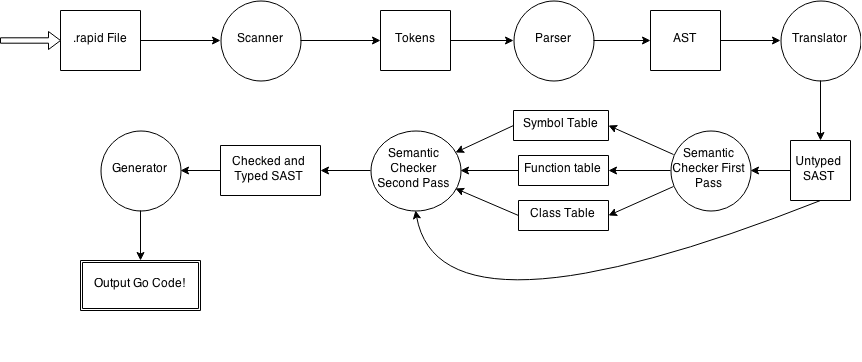
\includegraphics[scale=0.5]{arch_flow.png}

The compilation of Rapid to go is broken down into 5 stages:

\begin{enumerate}
\item Scanning
\item Parsing
\item Translating
\item Semantic Checking/Type Checking
\item Code Generation
\end{enumerate}


\subsection*{5.2 Scanning}

The scanner is written in \textbf{ocamllex} and takes a .rapid text file and converts it into a stream of tokens.  The tokens represent keywords, types, and identifiers in the rapid program.

\subsection*{5.3 Parsing}

The parser uses \textbf{ocamlyacc} to convert the tokens it receives from the scanner into and abstract syntax tree (AST).  The parser builds the AST as a list of statements, functions, classes and http trees.  Statements hold the kind of statement and associated expressions.  Functions hold a their name, a list of statements representing the variable declarations for the arguments, a list of statements representing the body and a list of statements. A class declaration has a list of it's members (Attributes or Functions). Finally an Http is a recursive tree here each no leaf node of the tree is a namespace block or a param block.  The leaves of the tree are http functions.  

\subsection*{5.4 Translation}

Translation gets the AST from the parser in the from of a tuple of AST Statements, AST Functions, AST HTTP trees and AST Classes.  Translation takes the AST and Translates it to an initial semantic abstract syntax tree (SAST). This SAST has the same structure as the AST.  At this step all literals are rewritten to typed expressions.  

\subsection*{5.5 Semantic Checking}

After translation the SAST is scanned for variable declarations, function declarations, and class declarations.  When one of these is found it is added to the symbol table, function table, or class respectively.  This pass must be done before semantic checking because functions and class do not have to be declared before being used.  Once these tables are built the SAST is walked once more to check types.  Expressions are recursively rewritten to typed expressions and then typed checked. In binary operations ints are marked for casting to float if they are found in a binary operator expression expecting a float.  Functions declarations are scanned for a return statement of the proper type.  Statements are check to make sure their expressions are of the correct type.  Class instantiations and function calls are check for the proper number and type of arguments they are passed.  Once all this type checking and rewriting is done the SAST is passed to the code generator.

\subsection*{5.6 Code Generation}

The code generator takes the SAST from the Semantic Checker and generates go code.  Because go has a main function and RAPID does not, we first pull out all the var declarations and write the go declarations before main. This is because these variables are global in our language. Now we recurse through each part of the SAST (statements, functions, classes, and http blocks) and write each part of them to code.  Because our language supports null values and go does not we use go pointers to represent all of our types.  This means that to generate functioning code statements have to be written in two parts.  First, temp variables are created in go and set to value of on part of the expression.  Then these temp values are used to evaluated the expression.  for example rapid code:
\begin{verbatim}
int x = 5; would get 
int i = x;
\end{verbatim}

Would generate the following go code:
\begin{verbatim}
//declarations pulled out
x Int //Int is type we defined as pointer to int.
i Int
//int x = 5; 
tmp = 5
x = &tmp
//int i = x;
tmp = *x
i = &tmp
\end{verbatim} 

\newpage

\section*{Test Plan and Scripts}
% TODO: fix this file
% \documentclass[]{article}
\usepackage{lmodern}
\usepackage{amssymb,amsmath}
\usepackage{ifxetex,ifluatex}
\usepackage{fixltx2e} % provides \textsubscript
\ifnum 0\ifxetex 1\fi\ifluatex 1\fi=0 % if pdftex
  \usepackage[T1]{fontenc}
  \usepackage[utf8]{inputenc}
\else % if luatex or xelatex
  \ifxetex
    \usepackage{mathspec}
    \usepackage{xltxtra,xunicode}
  \else
    \usepackage{fontspec}
  \fi
  \defaultfontfeatures{Mapping=tex-text,Scale=MatchLowercase}
  \newcommand{\euro}{€}
\fi
% use upquote if available, for straight quotes in verbatim environments
\IfFileExists{upquote.sty}{\usepackage{upquote}}{}
% use microtype if available
\IfFileExists{microtype.sty}{%
\usepackage{microtype}
\UseMicrotypeSet[protrusion]{basicmath} % disable protrusion for tt fonts
}{}
\usepackage{longtable,booktabs}
\ifxetex
  \usepackage[setpagesize=false, % page size defined by xetex
              unicode=false, % unicode breaks when used with xetex
              xetex]{hyperref}
\else
  \usepackage[unicode=true]{hyperref}
\fi
\hypersetup{breaklinks=true,
            bookmarks=true,
            pdfauthor={},
            pdftitle={},
            colorlinks=true,
            citecolor=blue,
            urlcolor=blue,
            linkcolor=magenta,
            pdfborder={0 0 0}}
\urlstyle{same}  % don't use monospace font for urls
\setlength{\parindent}{0pt}
\setlength{\parskip}{6pt plus 2pt minus 1pt}
\setlength{\emergencystretch}{3em}  % prevent overfull lines
\setcounter{secnumdepth}{0}

\date{}

\begin{document}

\section{RAPID Language Reference
Manual}\label{rapid-language-reference-manual}

\subsection{Coms W 4115}\label{coms-w-4115}

Ben Edelstein, Brian Shin, Brendon Fish, Dan Schlosser, Nate Brennand

\subsection{1. Introduction}\label{introduction}

With increased demand in the public and private sector for
cloud-connected mobile and web applications has come a rising need for
web servers to maintain state across multiple devices and users.
Development of web servers is complex, however. Building a web server
using modern web server packages requires learning a server-side
programming language, and then integrating a web server package and
implementing required methods. Furthermore, local testing and
development of these servers is excessively complex, as they have
numerous dependencies and are difficult to build.

RAPID is a programming language intended specifically for the rapid
development of modern web APIs. Using RAPID, developers can quickly
build a database-backed REST API server that guarantees JSON shapes in
responses. RAPID is object oriented and database-backed, meaning that
classes represent an SQL table, and upon instantiation objects are
automatically saved in the database. This abstracts away much of the
boiler plate code that developers typically write when building an API
server.

\subsubsection{1.1 Why RAPID?}\label{why-rapid}

The name RAPID represents the goal of the language: making API server
development quick. Also, it's a recursive acronym for \emph{RAPID
Application Programmer Interface Dialect}.

\subsubsection{1.2 RAPID Programs}\label{rapid-programs}

There are two types of RAPID programs, servers and scripts. If a program
contains an HTTP method, it is a server, otherwise it is a script. (See
more in later sections).

\subsection{2. Lexical Conventions}\label{lexical-conventions}

\subsubsection{2.1 Identifiers}\label{identifiers}

Identifiers must start with a letter or an underscore, followed by any
combination of letters, numbers, and underscores.

\begin{quote}
\textbf{Valid Identifiers:}

\texttt{abc}, \texttt{abc\_def}, \texttt{a\_\_\_1}, \texttt{\_\_a\_\_},
\texttt{\_1}, \texttt{ABC}
\end{quote}

\begin{quote}
\textbf{Invalid Identifiers:}

\texttt{123}, \texttt{abc-def}, \texttt{1abc},
\texttt{ab\textbackslash{} cd}
\end{quote}

\subsubsection{2.2 Keywords}\label{keywords}

The following identifiers are keywords in RAPID, and are reserved. They
can not be used for any other purpose.

\texttt{if}, \texttt{else}, \texttt{for}, \texttt{in}, \texttt{while},
\texttt{switch}, \texttt{case}, \texttt{default}, \texttt{fallthrough},
\texttt{http}, \texttt{func}, \texttt{json}, \texttt{class},
\texttt{namespace}, \texttt{param}, \texttt{true}, \texttt{false},
\texttt{new}, \texttt{optional}, \texttt{unsafe}, \texttt{instance},
\texttt{and}, \texttt{or}

\subsubsection{2.3 Literals}\label{literals}

\paragraph{Integer literals}\label{integer-literals}

Integer literals may be declared using digits.

\begin{verbatim}
int x = 5
\end{verbatim}

\paragraph{Float literals}\label{float-literals}

Float literals are declared as an integer part, a decimal point, and a
fraction part, all of which are mandatory. The integer part may not
start with a zero, unless it is only a zero (for floats less than
\texttt{1.0}), in which case it is still required. There may not be any
whitespace between these three parts.

\begin{verbatim}
// Valid float literals:
float x = 15.0
float y = 0.25

// Invalid float literals:
float z = .5
float w = 10.
float v = 1 . 4
\end{verbatim}

\paragraph{String literals}\label{string-literals}

String literals are declared using double quotes. Special characters may
be declared using the \texttt{\textbackslash{}} escape character.

\begin{verbatim}
string a = "hello"
string b = " \"world\"\n"
\end{verbatim}

\paragraph{Boolean literals}\label{boolean-literals}

Boolean literals are declared using the \texttt{true} and \texttt{false}
keywords.

\begin{verbatim}
boolean t = true
boolean f = false
\end{verbatim}

\paragraph{List literals}\label{list-literals}

List literals may be declared between square brackets, with
comma-separated values.

\begin{verbatim}
list<int> a = [1,2,3,4]
list<string> b = ["hello", "world"]
\end{verbatim}

\paragraph{Dictionary literals}\label{dictionary-literals}

Dictionary literals may be declared as comma-separated key value pairs
between braces, with a colon separating the key and value. Whitespace is
ignored.

\begin{verbatim}
dict<string, int> a = {"hello": 4, "world": 5}
dict<string, ing> b = {
    "a": 42,
    "b": 27
}
\end{verbatim}

\subsubsection{2.4 Comments}\label{comments}

There are two types of comments in RAPID: single line comments, and
block comments. Single line comments are preceded by \texttt{//} and
block comments begin with \texttt{/*} and end with \texttt{*/}

\begin{verbatim}
// This is a single line comment

/*
This is a multi-line
comment
/* They may be nested */
*/
\end{verbatim}

\subsubsection{2.5 Operators}\label{operators}

\begin{longtable}[c]{@{}clll@{}}
\toprule
Operator & Use & Associativity & Types\tabularnewline
\midrule
\endhead
\texttt{+} & Addition & left & int ,float\tabularnewline
\texttt{*} & Multiplication & left & int ,float\tabularnewline
\texttt{/} & Division & left & int ,float\tabularnewline
\texttt{-} & Subtraction & left & int ,float\tabularnewline
\texttt{\%} & Modulus & left & int\tabularnewline
\texttt{=} & Assignment & non-associative & All\tabularnewline
\texttt{==} & Equal to & non-associative & All\tabularnewline
\texttt{!=} & Not equal to & non-associative & All\tabularnewline
\texttt{\textgreater{}} & Greater than & non-associative & int,
float\tabularnewline
\texttt{\textless{}} & Less than & non-associative & int,
float\tabularnewline
\texttt{\textgreater{}=} & Greater than or equal to & non-associative &
int, float\tabularnewline
\texttt{\textless{}=} & Less than or equal to & non-associative & int,
float\tabularnewline
\texttt{and} & Logical And & non-associative & bool\tabularnewline
\texttt{or} & Logical Or & non-associative & bool\tabularnewline
\bottomrule
\end{longtable}

\subsection{3. Types}\label{types}

\subsubsection{3.1 Static Typing}\label{static-typing}

RAPID is a statically typed language; variables must be explicitly typed
upon declaration. Variables can be cast to other types (see Casting).

\subsubsection{3.2 Primitive Types}\label{primitive-types}

\paragraph{null}\label{null}

In RAPID, the \texttt{null} keyword represents an uninitialized value.
Any type in rapid may take on \texttt{null} if it hasn't been
initialized, or otherwise doesn't exist. The \texttt{null} keyword
represents a value, but null values are still typed. Null variables of
different types may not be assigned to each other, and may not be
compared. Null variables of the same type are equal. All variables will
\texttt{null} value are equal to the keyword \texttt{null}.

\begin{verbatim}
int x
int y = null
string s
boolean eq = (x == y) and (x == null) and (s == null)
x == s  // not valid RAPID
x = s   // not valid RAPID
\end{verbatim}

Null values of any type may not be used in operations together. If they
are, the program will exit prematurely, or the HTTP server will return a
500 error.

\begin{verbatim}
int x         // null
int y = x + 2 // not allowed, the program exits or the request returns 500.
list<int> a = [1, 2, 3, 4]
a[x]          // not allowed, the program exits or the request returns 500.
\end{verbatim}

\paragraph{Booleans}\label{booleans}

Boolean values are defined by the \texttt{true} and \texttt{false}
keywords. Because they are their own type, non-boolean values must be
cast to \texttt{boolean} in order to be used in logical expressions.

For example:

\begin{verbatim}
!(3+5)? // valid RAPID

!(3+5) // not valid RAPID
\end{verbatim}

The \texttt{?} is a an operator on all primitive types that evaluates to
the ``truthiness'' of that value.

\paragraph{Integers}\label{integers}

Integers are preceded by the type \texttt{int}, and represent an 8 byte,
signed integer. Integers can be declared and initialized later, or
initialized inline. Uninitialized integers are null.

\begin{verbatim}
int i     // null
int i = 5 // 5
\end{verbatim}

Integers are copied by value.

\begin{verbatim}
int a = 1
int b = a
a = 2
printf("%d, %d", a, b) // 2 1
\end{verbatim}

\paragraph{Floating Point Numbers}\label{floating-point-numbers}

Floating point numbers are preceded by the type \texttt{float}, and
represent IEEE-754 64-bit floating-point numbers.. They can be declared
and initialized later, or initialized inline.

\begin{verbatim}
float i        // null
float j = 3.14 // 3.14
\end{verbatim}

\paragraph{Strings}\label{strings}

Strings in RAPID are mutable, and declared with the \texttt{string}
type, and have the default value of the empty string. String literals
are declared using double quotes, and special characters may be escaped
using the \texttt{\textbackslash{}} character. Strings may be indexed
using square brackets. Because there is no Character type in RAPID,
single characters are strings of length 1. Multiline strings may be
declared using triple double quotes. Newlines are preserved and quotes
do not need to be escaped, but they may not be nested. Strings are pass
by value.

\begin{verbatim}
string s                      // null
string character = "c"        // c
string s = "He is \"Batman\"" // He called himself "Batman"
string c = s[0]               // H
string multi = """
Did you hear?

He calls himself "Batman".
"""                           // multi[0] => "\n"
\end{verbatim}

\subsubsection{3.3 Non-Primitive Types}\label{non-primitive-types}

\paragraph{List}\label{list}

The \texttt{list} type is a zero-indexed array that expands to fit it's
contents. The type of the contents must be provided within angle
brackets in the type signature. RAPID \texttt{list} literals may be
declared using square brackets, and values may be accessed or set using
square brackets. Uninitialized lists default to the empty list. Lists
are pass by reference.

\begin{verbatim}
/* List declaration */

list< /* type */ > /* id */ = [
    /* expression */,
    /* expression */,
    ...
    /* expression */
]
\end{verbatim}

\begin{verbatim}
list<int> empty // []
list<int> numbers = [1,2,3,42]
numbers[3]      // 42
numbers[1] = 5  // [1,5,3,42]
\end{verbatim}

\paragraph{Dictionary}\label{dictionary}

The \texttt{dict} type is similar to an object, but it's key set is
mutable. The type of the key and value must be provided within angle
brackets in the type signature. Only primitive types may be used as
keys. Keys may be added, set, and accessed using square brackets. RAPID
\texttt{dict} literals may be declared as comma-separated
\texttt{key:value} pairs surrounded by braces. Uninitialized
dictionaries default to the empty dictionary. Dictionaries are pass by
reference.

\begin{verbatim}
/* Dictionary declaration */

dict< /* type */ , /* type */ > /* id */ = {
    /* expression:string */ : /* expression */,
    /* expression:string */ : /* expression */,
    ...
    /* expression:string */ : /* expression */
}
\end{verbatim}

\begin{verbatim}
dict<string, int> empty // {}
dict<string, int> ages = {"Alice":3, "Bob":5}
ages["Alice"]           // 3
ages["Bob"] = 4         // {"Alice":3, "Bob":4}
ages["Caroline"] = 7    // {"Alice":3, "Bob":4, "Caroline":7}
\end{verbatim}

\paragraph{Object}\label{object}

The \texttt{object} type is a generic, non-primitive, dictionary-backed
type that has attributes for instance variables and functions. Accessing
instance variables or functions can be done with dot notation. Objects
may not be declared anonymously; they must be declared as instances of
classes. Objects have immutable key sets, so variables and functions may
not be added or removed, although their values may be changed. For more
on classes and instantiation, see Classes.

\paragraph{json}\label{json}

The \texttt{json} type is shares qualities of a dictionary and of an
Object. Every \texttt{json} type is directly connected to an Object
class that is user-defined. They have keys and values like dictionaries,
but have the strict requirements of shape like objects do. Every
property of a class is a mandatory key on the corresponding
\texttt{json} object, and properties that have default values on objects
have default values in \texttt{json}. Unlike objects, however,
\texttt{json} objects do not have methods associated with them, and
instances do not represent rows in the database. Each \texttt{class}
declaration defines an Object type and a \texttt{json} object type, and
only \texttt{json} objects that are associated with classes may be
instantiated.

For example, if we previously defined a \texttt{User} object with three
instance variables \texttt{username}, \texttt{full\_name}, and
\texttt{password} (all strings), then we may declare a \texttt{json}
User like so:

\begin{verbatim}
/* JSON Object initialization */

json< /* id:classname */ > /* id */ = json< /* id:classname */ >(
    key = /* expression */,
    key = /* expression */,
    ...
    key = /* expression */
)
\end{verbatim}

\begin{verbatim}
json<User> steve = json<User>(
    username="sedwards",
    full_name="Stephen Edwards",
    password="easypeasy"
)
\end{verbatim}

\paragraph{Errors}\label{errors}

Errors in RAPID are not thrown and caught, rather they are returned
directly by unsafe functions (see Functions).\\Errors contain a string
message, which can be dot-accessed, an integer error code that conforms
with the HTTP/1.1 standard, and an optional string name.

For example, to declare a custom error:

\begin{verbatim}
error e = error(message="There was an error with that Request.",
                code=400,
                name="RequestError")
\end{verbatim}

Unsafe operations return an error as the last return value:

\begin{verbatim}
dict<string, int> d = {"foo": 4, "bar": 5}
int val, error e = d["baz"]
if (!e?) {
    printf("%d\n", e.code)    // 500
    printf("%s\n", e.message) // Key error when accessing "baz" on `d`.
    printf("%s\n", e.name)    // KeyError
}
\end{verbatim}

Many standard library classes and builtin objects define errors
pertinent to their functions, to which an error instance may be
compared.

\begin{verbatim}
dict<string, int> d = {"foo": 4, "bar": 5}
int val, error e = d["baz"]
if (!e?) {
    printf("%s", e == dict.KeyError) // true
}
\end{verbatim}

\subparagraph{Stacking}\label{stacking}

Unsafe functions (like list and dictionary access) may exist in the same
expression. If unsafe functions return successfully, the error that is
returned is consumed (ignored), and the return value is taken. If an
unsafe function returns an error, the expression evaluation
short-circuits, and the value of the expression is null and the error
that is returned by the failed function call.

\begin{verbatim}
dict<string, list<int>> d = {"foo": [4,5], "bar": [1,2,3]}
int val, error e = d["foo"][2]     // List index out of bounds...
printf("%d", val)                  // null
printf("%s", e.name)               // IndexError
printf("%t", e == list.IndexError) // true

val, e = d["baz"][0]             // No such key, short circuit
printf("%d", val)                // null
printf("%s", e.name)             // KeyError
printf("%t", e == dict.KeyError) // true
\end{verbatim}

More generally, if a subexpression of an expression is unsafe, it is
presumed to be successful and the return value of the subexpression is
used in the evaluation of the larger expression, unless the unsafe
expression evaluates to an error, in which case evaluation of the large
expression short-circuits, and the value of the large expression is
\texttt{null, /* sub-expression\textquotesingle{}s error */}.

\subparagraph{Predefined Responses}\label{predefined-responses}

Unsafe functions may also choose to return an predefined response, which
is an predefined literal that will be cast to a generic error object at
compile time.\\See Functions for more details.

All predefined errors exist in the root scope and are named according to
their status code, \texttt{e\textless{}code\textgreater{}}.

\texttt{e404} is the error, \texttt{error("Not Found", 404, "NotFound")}
(message, code, name).\\All the below errors are predefined as such.

\begin{longtable}[c]{@{}llll@{}}
\toprule
Response & Message & Code & Name\tabularnewline
\midrule
\endhead
\texttt{e100} & Continue & 100 & \texttt{Continue}\tabularnewline
\texttt{e200} & OK & 200 & \texttt{OK}\tabularnewline
\texttt{e201} & Created & 201 & \texttt{Created}\tabularnewline
\texttt{e301} & Moved Permanently & 301 &
\texttt{MovedPermanently}\tabularnewline
\texttt{e302} & Found & 302 & \texttt{Found}\tabularnewline
\texttt{e304} & Not Modified & 304 & \texttt{NotModified}\tabularnewline
\texttt{e400} & Bad Request & 400 & \texttt{BadRequest}\tabularnewline
\texttt{e401} & Unauthorized & 401 &
\texttt{Unauthorized}\tabularnewline
\texttt{e403} & Forbidden & 403 & \texttt{Forbidden}\tabularnewline
\texttt{e404} & Not Found & 404 & \texttt{NotFound}\tabularnewline
\texttt{e405} & Method Not Allowed & 405 &
\texttt{MethodNotAllowed}\tabularnewline
\texttt{e410} & Gone & 410 & \texttt{Gone}\tabularnewline
\texttt{e413} & Request Entity Too Large & 413 &
\texttt{RequestEntityTooLarge}\tabularnewline
\texttt{e414} & Request-URI Too Long & 414 &
\texttt{RequestURITooLong}\tabularnewline
\texttt{e417} & Expectation Failed & 417 &
\texttt{ExpectationFailed}\tabularnewline
\texttt{e500} & Internal Server Error & 500 &
\texttt{InternalServerError}\tabularnewline
\texttt{e501} & Not Implemented & 501 &
\texttt{NotImplemented}\tabularnewline
\texttt{e502} & Bad Gateway & 502 & \texttt{BadGateway}\tabularnewline
\texttt{e503} & Service Unavailable & 503 &
\texttt{ServiceUnavailable}\tabularnewline
\texttt{e504} & Gateway Timeout & 504 &
\texttt{GatewayTimeout}\tabularnewline
\bottomrule
\end{longtable}

\paragraph{Functions}\label{functions}

Functions are first class objects, and may be passed around as variables
(see Functions)

\subsubsection{3.4 Casting}\label{casting}

\paragraph{Integers and Floats}\label{integers-and-floats}

Casting between float and int can be done using the \texttt{float()} and
\texttt{int()} keyword functions. Floats are floored when they are cast
to int. Additionally, integers are cast to floats if floats and integers
are used together in a binary operator.

\begin{verbatim}
float f = 7.5
int i = 3
float f = float(i) // f == 3.0
int i = int(f)     // i == 7
\end{verbatim}

When an int and a float are involved in a binary operator, the integer
will be cast to a float implicitly.

\begin{verbatim}
float f = 7.5 + 10    // 17.5
boolean eq = 4.0 == 4 // true
\end{verbatim}

\paragraph{Booleans}\label{booleans-1}

Any value may be cast to boolean using the \texttt{?} operator.

See the following table for the result of using the \texttt{?} operator
on various types:

\begin{longtable}[c]{@{}lccl@{}}
\toprule
Type & \texttt{true} & \texttt{false} & Comments\tabularnewline
\midrule
\endhead
boolean & \texttt{true?} & \texttt{false?} & Booleans retain their
value\tabularnewline
int & \texttt{1?}, \texttt{-1?} & \texttt{0?} & 0 is \texttt{false},
other ints are \texttt{true}\tabularnewline
float & \texttt{1.0?}, \texttt{-1.0?} & \texttt{0.0?} & 0.0 is
\texttt{false}, other floats are \texttt{true}\tabularnewline
null & - & \texttt{null?} & \texttt{null} is
\texttt{false}\tabularnewline
list & \texttt{{[}0{]}?}, \texttt{{[}false{]}?} & \texttt{{[}{]}?} &
Empty lists are \texttt{false}\tabularnewline
dict & \texttt{\{"key":false\}?} & \texttt{\{\}?} & Empty dicts are
\texttt{false}\tabularnewline
json & \texttt{json\textless{}Obj\textgreater{}()?} & - & JSON objects
are \texttt{true}\tabularnewline
object & \texttt{Obj()?} & - & Objects are \texttt{true}\tabularnewline
\bottomrule
\end{longtable}

\subsection{4. Database Backing}\label{database-backing}

\subsubsection{4.1 Classes}\label{classes}

RAPID classes are backed by a PostgreSQL database.\\Classes are defined
using the \texttt{class} keyword, and represent an SQL table.\\Instance
variables (variables declared directly within the \texttt{class} block)
represent columns for the table.\\Instances of a class represent rows in
SQL.\\By default, columns are not nullable, but this may be overwritten
using the \texttt{optional} keyword.\\If the assignment syntax is used,
a default value will be given.

\begin{verbatim}
class /* id */ {
    /* declaration */
    /* declaration */
    ...
    /* declaration */
}
\end{verbatim}

Take the following example:

\begin{verbatim}
class User {
    string username
    optional string full_name
    int age = 18
    string password
}
\end{verbatim}

In this example, the ``User'' table has four columns: \texttt{username},
\texttt{full\_name}, \texttt{age}, and \texttt{password}. The
\texttt{full\_name} column may be omitted in the instantiation, and if
\texttt{age} is omitted, it will take the value \texttt{18}.

\paragraph{Instance Methods}\label{instance-methods}

Instances of objects may have methods that operate on their instances
variables. Using the \texttt{instance} keyword, a block may be created
in which instance methods may be defined:

\begin{verbatim}
class /* id:classname */ {
    instance /* id:selfname */ {
        /* declaration */
        /* declaration */
        ...
        /* declaration */
    }
}
\end{verbatim}

The identifier specified after the \texttt{instance} keyword will
represent the instance in all functions defined inside the
\texttt{instance} block.

Instance methods may not be \texttt{http} routes. The \texttt{.} is
syntactic sugar for calling instance methods.

For example:

\begin{verbatim}
class User {
    string first_name
    string last_name

    instance my {
        func get_full_name() string {
            return my.first_name + " " + my.last_name
        }
    }
}

User obama = User(first_name="Barrak", last_name="Obama")
printf("%s", obama.get_full_name()) // Barrak Obama
\end{verbatim}

\paragraph{Instantiation}\label{instantiation}

New instances of a class may be declared using the \texttt{new}
keyword.\\The \texttt{new} keyword is followed by the name of the class
and a pair of parenthesis, in which a JSON User literal (described more
in-depth in the next section) may be passed to declare instance
variables.\\Once a user defined object is created, it will be database
backed.\\Any changes to the object will trigger an update to the
database backed copy.\\Every object will have an \texttt{ID} attribute
generated (this is a reserved attribute that cannot be used).\\This is a
unique identifier to the object.

\begin{verbatim}
User bob = new User(
    username="burgerbob",
    full_name="Bob Belcher",
    password="burgersrock",
    age=42
)
\end{verbatim}

\subsubsection{Deletion}\label{deletion}

All objects have an instance method, \texttt{delete()}, defined that
will delete the database record.\\There is no return value for the
\texttt{delete} call.

\paragraph{json}\label{json-1}

Defining the ``User'' class defines a \texttt{User} type, as well as a
\texttt{json\textless{}User\textgreater{}} type. The
\texttt{json\textless{}User\textgreater{}} type has the same keys and
value types as the User class, and may be declared in dictionary literal
syntax.

\begin{verbatim}
json<User> bob_json = json<User>(
    username="burgerbob",
    full_name="Bob Belcher",
    password="burgersrock",
    age=42
)
\end{verbatim}

This \texttt{json\textless{}User\textgreater{}} object does not
represent a row in the database, and will be deallocated when it leaves
scope.

It may be passed into an instantiation statement for a User object, to
be persisted:

\begin{verbatim}
User bob, error e = new User(bob_json)
\end{verbatim}

\subsubsection{4.2 Querying}\label{querying}

Objects may be queried from the database using the \texttt{get}
function, which is automatically defined on all classes.\\\texttt{get}
is an unsafe function which will return a list of objects as well as an
error.

The following example queries all User objects from the database:

\begin{verbatim}
Tweet[] tweets = Tweet.get()
\end{verbatim}

A optional \texttt{filter} parameter can be set to limit the responses
returned by Get().\\The filter value shoudld be a dictionary of
attributes and values.\\Any non-existant attributes in the dictionary
will be logged as an warning and ignored.

\begin{verbatim}
// returns all tweets by burgerbob.
Tweet[] tweets, error e = Tweet.get(filter={
  username="burgerbob"
})
\end{verbatim}

A optional \texttt{ID} parameter can be set to return a single
Object.\\This can be combined with filter if desired.

In the case that the object is not found, the returned object will be
\texttt{null} and the error will be a non-null value.

\begin{verbatim}
// returns all tweets by burgerbob.
Tweet t, error e = Tweet.get(ID="123abc")
\end{verbatim}

\subsubsection{4.3 Updates}\label{updates}

\subsection{5. Functions}\label{functions-1}

\subsubsection{5.1 Declaration}\label{declaration}

Functions in RAPID are first-class objects, but may not be declared
anonymously. Functions are declared using the \texttt{func} keyword. The
arguments (within parenthesis), return type (after the parenthesis, but
before the braces), and the body of the function (within the braces)
must be declared explicitly. Return types may include multiple types
separated by commas, or may be omitted for void functions.

Return values are specified using the \texttt{return} keyword, which
must be followed by an expression to be returned for functions that have
declared return types. If the return type is omitted, the function is
void, and the result of calling it may not be assigned to a value. Void
functions may use the \texttt{return} keyword by itself to exit
prematurely from the function.

Unsafe functions may not be void, because they must return errors.

\begin{verbatim}
return /* expression */
\end{verbatim}

The arguments must be in order \texttt{namespace} arguments, then formal
arguments. Arguments may be given a literal default value, using an
equal sign, but all arguments with default values must follow arguments
without default values.

\begin{verbatim}
[unsafe] func /* id */ ( /* namespace args */ /* formal args */ ) /* return type*/ {
    // statements
}
\end{verbatim}

For example:

\begin{verbatim}
func sum(int a, int b=1) int {
    return a + b
}
sum(5) //
\end{verbatim}

Or:

\begin{verbatim}
func printInt(int a) {
    printf("%d", a)
}
\end{verbatim}

\subsubsection{5.2 Unsafe Functions}\label{unsafe-functions}

If a function performs actions that may be unsafe, it must be preceded
by the keyword \texttt{unsafe}. Unsafe functions return unsafe
expressions, which is denoted by the presence of an \texttt{error}-typed
second value that is returned.

\begin{verbatim}
unsafe func access(dict<string, int> d, string key) int {
    int val, error error = d[key]
    return val, error
}
\end{verbatim}

Notice that the return type remains \texttt{int}, although an error is
also returned. For more on unsafe expressions, see Expressions.

Unsafe functions may also return a error, which are integer literals
that will be cast to a generic error object at compile time. See Status
Code Definitions for a complete list of error codes that may be declared
as anonymous errors.

\begin{verbatim}
/* Default dict accessing:
 *    If there is a KeyError, return 0 with a 400 Not Found error
 */
unsafe func access(dict<string, int> d, string key) int {
    int val, error error = d[key]
    if (error == dict.KeyError) {
        return 0, e400
    }
    return val, e200
}
\end{verbatim}

\subsection{6. Routing}\label{routing}

One of the core features of RAPID is it's ability to easily define
routes for a REST API server.

\subsubsection{6.1 Declaring Routes}\label{declaring-routes}

Routes may be declared like functions, but substituting the
\texttt{http} keyword for the \texttt{func} keyword. Routes specify a
REST API endpoint, it's parameters, it's response, and any side effects.

Like functions, routes take namespace arguments, and then other formal
arguments. Unlike functions, however, routes may also take a single
request body argument that of a
\texttt{json\textless{}Obj\textgreater{}} type. It will be read from the
request body and interpreted as JSON.

\begin{verbatim}
http /* id */ ( /* namespace args */ /* formal args */ /* request body args */) {
    // statements
}
\end{verbatim}

Routes are unsafe by default, and therefore must include \texttt{error}
in their return types. This may be an anonymous error (see Functions).

For example, the following route echos the URL parameter that it is
passed.

\begin{verbatim}
http echo(string foo) string, error {
    return foo, e200
}
\end{verbatim}

The name of the function will be the name of the route. Therefore, in
the preceding example, a \texttt{GET} request to \texttt{/echo?foo=Dog}
will return \texttt{"Dog"}.

\subsubsection{6.2 Path context}\label{path-context}

The endpoint associated with each route is determined by the combination
of one or more blocks associated with it and the name of the route
itself. There is a one-to-one mapping from any route to a series of
accessors on class instances.

\paragraph{Classes}\label{classes-1}

Classes provide path context. Class names are put to lowercase, and
appended to path context. The following example defines a route named
\texttt{add} inside a class called \texttt{Math}.

\begin{verbatim}
class Math {
    http add(int a, int b) int {
        return a + b, e200
    }
}
\end{verbatim}

A \texttt{GET} request to \texttt{/math/add?a=3\&b=4} will return
\texttt{7}.

Similarly, the following code will print \texttt{7}:

\begin{verbatim}
math = Math()
int sum, error _ = math.add(3,4)
printf("%d", sum)
\end{verbatim}

\paragraph{Namespaces}\label{namespaces}

Sometimes, functions or routes should be grouped together for
organization purposes, rather than any functional purpose. The
\texttt{namespace} keyword defines a named block of functions that has
the namespace name appended to the path context for those functions.

\begin{verbatim}
/* Namespace declaration */

namespace /* id */ {
    // statements
}
\end{verbatim}

\begin{verbatim}
class Math {
    namespace ops {
        http add(int a, int b) int { return a + b, e200 }
        http sub(int a, int b) int { return a - b, e200 }   
    }
    namespace convert {
        func ft_to_in(float feet) float { return feet*12, e200 }    
    }
}
\end{verbatim}

This defines routes at \texttt{/math/ops/add} and
\texttt{/math/ops/sub}, and functions at \texttt{Math.ops.add},
\texttt{Math.ops.sub}, and \texttt{Math.convert.ft\_to\_in}.

A \texttt{GET} request to \texttt{/math/ops/add?a=3\&b=4} will return
\texttt{7}.

\paragraph{Parameters}\label{parameters}

Variable URL parameters may be defined similar to namespaces, using a
named block with the \texttt{param} keyword. The \texttt{param} keyword
is followed by a type and an identifier.

Any function or route defined within a \texttt{param} block must take
the parameters defined by the \texttt{param} blocks in order from inside
to out.

\begin{verbatim}
param /* type */ /* id */ {
    // statements
}
\end{verbatim}

For example:

\begin{verbatim}
class Math {
    param int a {
        param int b {
            http add(int a, int b) int { return a + b, e200 }
        }   
        http square(int a) int { return a*a, e200 }
    }
}
\end{verbatim}

A \texttt{GET} request to \texttt{/math/5/7/add} will return
\texttt{12}, and a \texttt{GET} request to \texttt{/math/5/square} will
return \texttt{25}. A \texttt{GET} request to \texttt{/math/5/7/add?a=4}
will return return a 400 HTTP error. The following code snipped will
print \texttt{12} then \texttt{25}:

\begin{verbatim}
math = Math()
int sum, error _ = math.add(5,7)
printf("%d", sum)
int sqr, error _ = math.square(5)
printf("%d", sqr)
\end{verbatim}

\subsection{7. Syntax}\label{syntax}

\subsubsection{7.1 Program Structure}\label{program-structure}

A valid RAPID program is a series of valid statements. If the program
contains any \texttt{http} blocks, it will be interpreted as a restful
web API, and will run a HTTP web server on \texttt{localhost:5000}.

\subsubsection{7.2 Expressions}\label{expressions}

Expressions are series of operators and operands that may be evaluated
to a value and type. Any subexpressions are evaluated from left to
right, and side effects of evaluations occur by the time the evaluation
is complete. Type checking on operations occur in compile time.

\paragraph{Literals}\label{literals-1}

Literals may be of type string, integer, float, boolean, dict, or list.
See Lexical Conventions for more information.

\paragraph{Identifiers}\label{identifiers-1}

Identifiers could be primitive types, lists, dictionaries, objects, JSON
objects, functions, classes, or errors.

If an identifier represents a primitive type, list, dictionary, object,
JSON object, or error, it may be reused once per block.

For example, in the following example, the variable \texttt{a} changes
value three times.

\begin{verbatim}
float a = 4.5            // `a` is a float
func add(int a, int b) { // `a` is an int 
    return a + b         // the float `a` does not exist in this scope.
} 
string a = ""            // invalid RAPID, cannot rename 
                         // variables within the same scope.
\end{verbatim}

Identifiers are tied to the scope that they are declared in. The
following example prints \texttt{3}, then \texttt{5}, then \texttt{3}:

\begin{verbatim}
int a = 3
if (true) {
    printf("%d", a) // `a` is from the parent scope.
    int a = 5
    printf("%d", a) // `a` is from the local scope.
}
printf("%d", a) // the `a` from within the block does not leave it
\end{verbatim}

\paragraph{Binary Operators}\label{binary-operators}

Binary operators have two operands, one on the left side, and one on the
right.

\begin{verbatim}
/* expression */ /* bin-op */ /* expression */
\end{verbatim}

In the case of multiple consecutive binary operations without
parenthesis, the association of the binary operator is followed (see
Operators).

\paragraph{Parenthesized Expressions}\label{parenthesized-expressions}

Parenthesis may be used to alter the order of operand evaluation.

\subsubsection{7.3 Statements}\label{statements}

\paragraph{Assignments}\label{assignments}

Assignments have an \texttt{lvalue}, and an expression, separated by an
equal sign. Possible \texttt{lvalue}s include identifiers, accessors
(either list, dict, or object), a declaration, or another assignment:

\begin{verbatim}
/* lvalue */ = /* expression */
\end{verbatim}

Examples include:

\begin{verbatim}
a = b
int i = 7
j = square(i)
k = 5 * b
\end{verbatim}

\paragraph{Declarations}\label{declarations}

A declaration may be the declaration of a variable, an assignment, or
the declaration of a function, route, class, namespace, or param.

\subparagraph{Variable Declaration}\label{variable-declaration}

A variable declaration consists of a type and an id. A variable declared
in a scope block is accessible at every line following the line of its
declaration.

\begin{verbatim}
/* type */ /* id */
\end{verbatim}

\subparagraph{Function Declaration}\label{function-declaration}

The declaration of a function is a valid statement (see Functions).
Functions defined in a scope are accessible from anywhere in that scope.
Functions may call each other mutually independant of definition order.

\subparagraph{Route Declaration}\label{route-declaration}

The declaration of a class is a valid statement (see Routing). Like
functions, routes declared in a scope are accessible from anywhere in
that scope.

\subparagraph{Class Declaration}\label{class-declaration}

The declaration of a class is a valid statement (see Classes). Like
functions, classes declared in a scope are accessible from anywhere in
that scope.

\subparagraph{Namespace or Parameter
Declaration}\label{namespace-or-parameter-declaration}

The declaration of a namespace or parameter is a valid statement (see
Path Context). Like functions, namespces or parameters declared in a
scope are accessible from anywhere in that scope.

\paragraph{Function call}\label{function-call}

A function call is an identifier of a declared function and a set of
parenthesis containing the comma-separated arguments. There may not be a
space between the identifier and the open parenthesis. Function
arguments may be referenced by name, independent of whether or not the
argument has a default value. When arguments are referenced in the
function call by name, they may be rearranged, but may not be placed
before arguments that are not referenced by name.

\begin{verbatim}
func sub(int a=2, int b=1) int { return a - b }
int x = sub()         // 1
int y = sub(4, 2)     // 2
int z = sub(b=5, a=2) // 3
int w = sub(7, b=3)   // 4
int f = sub(a=3, 2)   // Not valid RAPID
\end{verbatim}

\paragraph{Control flow}\label{control-flow}

\subparagraph{If}\label{if}

If the expression between the parenthesis of an \texttt{if} statement
evaluates to \texttt{true}, then the statements within the body are
executed. Note that non-boolean values will not be cast to boolean, and
will result in a compile-time error.

\begin{verbatim}
if (/* expression */) { /* statements */ }
\end{verbatim}

\subparagraph{If-else}\label{if-else}

An \texttt{if} statement may be immediately followed by an \texttt{else}
statement, in which case the block of code within the braces after the
\texttt{else} keyword will be executed if the \texttt{if}'s expression
evaluates to \texttt{false}.

\begin{verbatim}
if (/* expression */) {
    // statements
}
else {
    // statements
}
\end{verbatim}

\subparagraph{Else-if}\label{else-if}

An \texttt{if} statement may be followed by an \texttt{else if}
statement, in which case the the second \texttt{if} statement will be
evaluated if and only if the first \texttt{if} statement evaluates to
\texttt{false}. The body of the \texttt{else if} is executed if the
second \texttt{if} statement is evaluated, and evaluates to
\texttt{true}. An \texttt{else if} statement may be followed by another
\texttt{else if} statement, or an \texttt{else} statement.

\begin{verbatim}
if (/* expression */) {
    // statements
}
else if (/* expression */) {
    // statements
}
...
else if (/* expression */ ) {
    // statements
}
else {
    // statements
}
\end{verbatim}

\subparagraph{Switch}\label{switch}

A \texttt{switch} statement includes an expression, which is evaluated
and then compared in order to a series of one or more \texttt{case}
expressions. If the expressions are equal, the body of the \texttt{case}
statement that matches will be executed, and then the switch statement
will short circuit. The \texttt{fallthrough} keyword may be used to
avoid this short circuit, continuing to compare the \texttt{switch}
expression with subsequent \texttt{case} expressions.

The \texttt{default} statement may be included after all \texttt{case}
statements, and will be executed if it is reached. This can be thought
of as a \texttt{case} whose expression always equals that of the
\texttt{switch}. Observe the syntax below:

\begin{verbatim}
switch (/* expression */) {
    case (/* expression */) {
        // statements
        fallthrough
    }
    case (/* expression */) {
        // statements
    }
    default {
        // statements
    }
}
\end{verbatim}

\paragraph{While loops}\label{while-loops}

While loops contain an expression and a body. If the expression
evaluates to \texttt{true}, the body will be executed. Afterwards, the
expression will be evaluated again, and the process repeats. Like
\texttt{if} statements, \texttt{while} statements must have expressions
that evaluate to a boolean in order to compile.

\begin{verbatim}
while (/* expression */) {
    // statements
}
\end{verbatim}

\paragraph{For loops}\label{for-loops}

A \texttt{for} loop may be used to iterate over a \texttt{list}. The
syntax is:

\begin{verbatim}
for (/* type */ /* id */ in /* list expr */) {
    // statements
}
\end{verbatim}

For example:

\begin{verbatim}
list<int> my_list = [1,2,3,4,5]
for (int num in my_list) {
    printf("%d ", num)
}
// 1 2 3 4 5
\end{verbatim}

The \texttt{range()} function in the standard library may be used to
generate lists of sequential integers.

\begin{verbatim}
for (int num in range(1,6)) {
    printf("%d ", num)
}
// 1 2 3 4 5
\end{verbatim}

\paragraph{Return statements}\label{return-statements}

A \texttt{return} statement may be used to exit a function, optionally
passing the value of an expression as the return value of the function.

\begin{verbatim}
return /* optional expression */
\end{verbatim}

For example:

\begin{verbatim}
func int add(int x, int y) int {
    return x + y
}
printf("%d", add(3,4))
// 7
\end{verbatim}

\paragraph{Break Statements}\label{break-statements}

A \texttt{break} statement can be used to exit a loop prematurely.

\begin{verbatim}
while (/* expression */) {
    break
}
\end{verbatim}

In the case of nested loops, the \texttt{break} statement only breaks
the loop in which it is stated.

\begin{verbatim}
while (/* expression */) {
    while (/* expression */) {
        break /* only breaks inner loop */
    }
}
\end{verbatim}

\subsection{8. Built-in Functions}\label{built-in-functions}

\subsubsection{8.1 length()}\label{length}

\begin{verbatim}
func length(string s) int
func length(list<T> l) int
func length(dict<T,S> d) int
func length(json<T> j) int
\end{verbatim}

Returns the length of the argument. For strings, this is the number of
characters in the string, for lists, this is the number of elements in
the list. For dictionaries, this is the number of keys, for JSON
objects, this is the number of keys.

Examples:

\begin{verbatim}
length("hello")                                // 5
length([0,1,2,3])                              // 4
length({"a":0, "b":null, "c": False, "d": ""}) // 4
\end{verbatim}

Taking the \texttt{length} of a \texttt{null} value will return
\texttt{null}

\subsubsection{8.2 range()}\label{range}

\begin{verbatim}
func range(int stop) int[]
func range(int start, int stop[, int step=1]) int[]
\end{verbatim}

Returns a list of integers \texttt{r} where
\texttt{r{[}i{]} = start + step*i} where \texttt{i\textgreater{}=0} and
while \texttt{r{[}i{]} \textless{} stop}. If start is omitted, it
defaults to 0. If step is omitted, it defaults to 1.

Step may be negative, in which\\case
\texttt{r{[}i{]} \textgreater{} stop}

Examples:

\begin{verbatim}
range(5)       // [1,2,3,4,5]
range(4,5)     // [4]
range(3,7,2)   // [3,5]
range(10,4,-2) // [10,8,6]
\end{verbatim}

\subsubsection{8.3 Output Functions}\label{output-functions}

There are four methods of outputing from the server.\\They all accept a
format string as the first argument and optional additional arguments
for format strings.

\paragraph{Print Functions}\label{print-functions}

\begin{itemize}
\itemsep1pt\parskip0pt\parsep0pt
\item
  \texttt{printf(String formatStr, {[}values{]})}
\end{itemize}

\texttt{printf} does not include a newline at the end of the
output.\\The output is directed to STDOUT.

\subsubsection{Logging Functions}\label{logging-functions}

\begin{itemize}
\itemsep1pt\parskip0pt\parsep0pt
\item
  \texttt{log.info(String formatStr, {[}values{]})}
\item
  \texttt{log.warn(String formatStr, {[}values{]})}
\item
  \texttt{log.error(String formatStr, {[}values{]})}
\end{itemize}

All output is preceded by a timestamp.\\The logging functions print with
a newline at the end.\\The output is directed to STDERR.

The method name being called precedes the message in all caps.

\begin{verbatim}
log.info("Hello, %s", "world")
// 2009/11/10 23:00:00 INFO: Hello, world
\end{verbatim}

\subsection{9. Standard Library}\label{standard-library}

\subsubsection{9.1 string}\label{string}

\paragraph{string.is\_empty()}\label{string.isux5fempty}

\begin{verbatim}
func is_empty() boolean
\end{verbatim}

Returns a boolean value of whether the string on which it is called is
of length 0 or \texttt{null}.

Examples:

\begin{verbatim}
string a = "dog"
string b = ""

a.is_empty()  // false
b.is_empty()  // true
\end{verbatim}

\paragraph{string.substring()}\label{string.substring}

\begin{verbatim}
unsafe func substring(start, stop) string
\end{verbatim}

Returns the substring of a string at the given indexes. The start and
stop indexes are inclusive and exclusive respectively. Providing
improper indexes will cause the function to throw an error (both must be
0 \textless{}= i \textless{}= length(s))

\begin{verbatim}
string a = "catdog"

string sub, error e = a.substring(1,4)   // "atd", null
string sub, error e = a.substring(3,99)  // null, error
string sub, error e = a.substring(50,99) // null, error
\end{verbatim}

\paragraph{Get (c = string{[}i{]})}\label{get-c-stringi}

Strings may be indexed using brackets. Inside the brackets must be a
zero-indexed integer. Getting is unsafe, and returns
\texttt{string, error}.

Examples:

\begin{verbatim}
string a = "catdog"

printf("%s", a[3]) // prints d
\end{verbatim}

\paragraph{Set (string{[}i{]} = s)}\label{set-stringi-s}

After indexing, an assignment may occur, to set a value of the list.
Setting is \texttt{unsafe} due to the possiblity of index errors, and
returns \texttt{string, error}.

Examples:

\begin{verbatim}
string a = "catdog"
a[2], error e = "p"
if (!e?) {
    printf("%s", a)
}
// prints capdog
\end{verbatim}

\paragraph{Iterate (c in string)}\label{iterate-c-in-string}

Strings may be iterated over in for loops. Each element is returned in
order.

Examples:

\begin{verbatim}
string a = "catdog"
for (string c in a) {
    printf("%s", c)
}
// prints catdog
\end{verbatim}

\paragraph{Slice (string{[}i:j{]})}\label{slice-stringij}

Strings may be sliced into substrings using slicing with brackets.
Slicing is \texttt{unsafe}, and returns \texttt{string, error}. Note
that unlike for \texttt{list.substring}, the second index of a slice may
be larger than the length of the string.

\begin{verbatim}
string a = "catdog"

a[1:4]    // "atd"
a[3:99]   // "dog"
a[50:99]   // error
\end{verbatim}

\subsubsection{9.2 list}\label{list-1}

\paragraph{list.is\_empty()}\label{list.isux5fempty}

\begin{verbatim}
func is_empty() boolean
\end{verbatim}

Returns whether the list on which it is called is empty.

\begin{verbatim}
list<int> a = []
list<int> b = [3,4]

a.is_empty()    // false
b.is_empty()    // true
\end{verbatim}

\paragraph{list.append()}\label{list.append}

\begin{verbatim}
func append(T elem) list<T>
\end{verbatim}

Appends the argument to the end of a list.\\The list is returned which
allows for chaining of \texttt{append} calls but the function has side
effects and does not need to be used in an assignment.

\begin{verbatim}
list<int> a = []

a.append(7)     // [7]
a.append(3)     // [7,3]
\end{verbatim}

\paragraph{list.pop()}\label{list.pop}

\begin{verbatim}
unsafe func pop() T
\end{verbatim}

Removes the last element in a list, and returns it. If the list is
empty, an error is returned.

\begin{verbatim}
list<int> a = [3,4]

a.pop()   // 4
a.pop()   // 3
a.pop()   // error
\end{verbatim}

\paragraph{list.push()}\label{list.push}

\begin{verbatim}
func push(T elem) list<T>
\end{verbatim}

\paragraph{list.concat()}\label{list.concat}

\begin{verbatim}
func concat(list<T> l) list<T>
\end{verbatim}

\paragraph{list.reverse()}\label{list.reverse}

\begin{verbatim}
func reverse() list<T>
\end{verbatim}

Reverses the list on which it is called and returns the reversed list.

\begin{verbatim}
list<int> a = [1,2,3,4,5]

a.reverse()  // [5,4,3,2,1]
\end{verbatim}

\paragraph{list.copy()}\label{list.copy}

Copies by the list value.

\begin{verbatim}
func copy() list<T>
\end{verbatim}

Returns a copy by value of the list on which it is called

\begin{verbatim}
list<int> a = [1,2,3,4,5]   // [1,2,3,4,5]
\end{verbatim}

\paragraph{Get (list{[}i{]})}\label{get-listi}

Lists may be indexed using brackets. Inside the brackets must be a
zero-indexed integer. Getting is unsafe, and for a
\texttt{list\textless{}T\textgreater{}} returns \texttt{T, error}

Examples:

\begin{verbatim}
list<int> a, error E = [1,2,3,4]
printf("%d", a[2])
\end{verbatim}

\paragraph{Set (list{[}i{]} = j)}\label{set-listi-j}

After indexing, an assignment may occur, to set a value of the list.
Setting is \texttt{unsafe}, and for a
\texttt{list\textless{}T\textgreater{}} returns \texttt{T, error}.

Examples:

\begin{verbatim}
list<int> a = [1,2,3,4]
a[2], error e = 5
if (!e?) {
    for (int i in a) {
        printf("%d", i)
    } 
}
// prints 1254
\end{verbatim}

\paragraph{Iterate (j in list)}\label{iterate-j-in-list}

Lists may be iterated over in for loops. Each element is returned in
order.

Examples:

\begin{verbatim}
list<int> a = [1,2,3,4]
for (int i in a) {
    printf("%d", i)
} 
// prints 1234
\end{verbatim}

\paragraph{Slice (list{[}i:j{]})}\label{slice-listij}

Lists may be sliced into sub-lists using slicing with brackets. Slicing
is \texttt{unsafe}, and for a \texttt{list\textless{}T\textgreater{}}
returns \texttt{list\textless{}T\textgreater{}, error}.

\begin{verbatim}
list<int> a = [1,2,3,4]
list<int> b, error e = a[2:4]
if (!e?) {
    for (int i in a) {
        printf("%d", i)
    } 
}
// prints 234
\end{verbatim}

\subsubsection{9.3 dict}\label{dict}

\paragraph{dict.is\_empty()}\label{dict.isux5fempty}

\begin{verbatim}
func is_empty() boolean
\end{verbatim}

Returns a boolean value of whether the dictionary on which it is called
is empty.

\begin{verbatim}
dict<string, string> d = {"Dog" : "cat"}
dict<string, string> e = {}

d.is_empty()    // false
e.is_empty()    // true
\end{verbatim}

\paragraph{dict.has\_key()}\label{dict.hasux5fkey}

\begin{verbatim}
func has_key(T key) boolean
\end{verbatim}

Returns a boolean value corresponding to whether the dictionary on which
it is called contains argument as a key.

\begin{verbatim}
dict<string, string> d = {"Dog" : "cat"}

d.has_key("Dog")  // true
d.has_key("Cow")  // false
\end{verbatim}

\paragraph{dict.insert()}\label{dict.insert}

\begin{verbatim}
func insert(T key, S value)
\end{verbatim}

Inserts the arguments as a key, value pair in the dictionary on which it
is called.

\begin{verbatim}
dict<string, string> d = {"Dog" : "cat"}

d.insert("Cow" : "Pig")  // {"Dog" : "cat", "Cow" : "Pig"}
 
\end{verbatim}

\paragraph{dict.remove()}\label{dict.remove}

\begin{verbatim}
unsafe func remove(T key)
\end{verbatim}

Removes the value for the key given in the argument from the dictionary
on which the function is called.

\begin{verbatim}
dict<string, string> d = {"Dog" : "cat", "Cow" : "Pig"}

d.remove("Dog")    // {"Cow" : "Pig"}
\end{verbatim}

\paragraph{dict.keys()}\label{dict.keys}

\begin{verbatim}
func keys() list<T>
\end{verbatim}

Returns a list of all keys in the dictionary on which it is called. The
type of the returned list is that of the type of the keys in the
dictionary.

\begin{verbatim}
dict<string, string> d = {"Dog" : "cat", "Cow" : "Pig"}

d.keys()    // ["Dog", "Cow"]
\end{verbatim}

\paragraph{dict.values()}\label{dict.values}

\begin{verbatim}
func values() list<S>
\end{verbatim}

Returns a list of all values for the keyset in the dictonary on which it
is called. The type of the returned list is that of the type of the
values in the dictionary.

\begin{verbatim}
dict<string, string> d = {"Dog" : "cat", "Cow" : "Pig"}

d.values()      // ["Cat", "Pig"]
\end{verbatim}

\paragraph{Get (dict{[}k{]})}\label{get-dictk}

Lists may be indexed using brackets. Inside the brackets must be a key
in the dictionary. Getting is \texttt{unsafe}, and for a
\texttt{dict\textless{}S,T\textgreater{}} returns \texttt{T, error}.

Examples:

\begin{verbatim}
dict<string, int> d = {"a":1, "b":2}
Int v, error e = d["a"]
if (!e?) {
    printf("%d", v)
}
// prints 1
\end{verbatim}

\paragraph{Set (dict{[}k{]} = v)}\label{set-dictk-v}

After indexing, an assignment may occur, to set a value of the list.

Examples:

\begin{verbatim}
dict<string, int> d = {"a":1, "b":2}
d["a"] = 5
printf("%d", d["a"]) 
// prints 5
\end{verbatim}

\paragraph{Iterate (j in dict)}\label{iterate-j-in-dict}

Lists may be iterated over in for loops. Each element is returned in
order.

Examples:

\begin{verbatim}
dict<string, int> d = {"a":1, "b":2}
for (int k, v in d) {
    printf("%s:%s, ", k, v)
} 
// prints a:1, b:2, 
\end{verbatim}

\subsubsection{9.4 error}\label{error}

\paragraph{error.message}\label{error.message}

\begin{verbatim}
string message
\end{verbatim}

Returns the value of the error message on for the error object on which
it is called.

\begin{verbatim}
error e = error(message="There was an error with that Request.",
                code=400,
                name="RequestError")

e.message       // "There was an error with that Request."
\end{verbatim}

\paragraph{error.code}\label{error.code}

\begin{verbatim}
int code
\end{verbatim}

Returns the value of the error message on for the error object on which
it is called.

\begin{verbatim}
error e = error(message="There was an error with that Request.",
                code=400,
                name="RequestError")

e.code      // 400
\end{verbatim}

\paragraph{error.name}\label{error.name}

\begin{verbatim}
string name
\end{verbatim}

Returns the value of the error message on for the error object on which
it is called.

\begin{verbatim}
error e = error(message="There was an error with that Request.",
                code=400,
                name="RequestError")

e.name      // "RequestError"
\end{verbatim}

\subsection{10. Program Execution}\label{program-execution}

RAPID programs compile to a Go executable which is a platform specific
binary.\\Statements will be executed in order of their declaration.\\If
a RAPID program contains an \texttt{http} route, then running the
executable will start a server on \texttt{localhost:5000} after all
statements are executed.

\paragraph{Flags}\label{flags}

There are several flags to customize the runtime of the app.

\begin{itemize}
\itemsep1pt\parskip0pt\parsep0pt
\item
  \texttt{-D \textless{}pg\_url\textgreater{}} : a string of ``:@/''.
  This is used to connect to the postgres server
\item
  \texttt{-L \textless{}filename\textgreater{}} : log output will be
  appended to the specified file, defaults to \texttt{server.log}
\item
  \texttt{-P \textless{}port\textgreater{}} : alters the port the
  service will run on, defaults to 80
\item
  \texttt{-H} : prints all the options available
\item
  \texttt{-V} : verbosely logs every HTTP request and the return values.
\end{itemize}

\end{document}
 \newpage

\section*{Conclusions}
\input{conclusion}
\newpage

\section*{Full Code Listing}
\input{code}
\newpage


\end{document}

